% ==============================================================================
% Main entry point for the VNU-UET Data Mining Report (XeLaTeX + BibTeX)
% ==============================================================================

\documentclass[a4paper,12pt,oneside]{report}

% Load official VNU-UET typography, margins, headings, and helper environments
% ==============================================================================
% Official VNU-UET Report / Thesis Style Preamble (XeLaTeX)
% Follows VNU-UET formatting guidelines & Data Mining course specifications:
%   - Font: Times New Roman (Unicode), 13pt body text
%   - Line spacing: 1.3 lines, parindent 1cm (with indentfirst), parskip 6pt
%   - Margins: top 2.5cm, bottom 3.0cm, left 3.0cm, right 2.0cm
% ==============================================================================

% Font configuration under XeLaTeX with graceful fallback for Overleaf Linux
\usepackage{fontspec}
\IfFontExistsTF{Times New Roman}{
    \setmainfont{Times New Roman}
}{
    \setmainfont{TeX Gyre Termes}
}

% Official VNU-UET page geometry (left 3cm for binding, right 2cm, top 2.5cm, bottom 3cm)
\usepackage[
    a4paper,
    top=2.5cm,
    bottom=3.0cm,
    left=3.0cm,
    right=2.0cm,
    footskip=1.2cm
]{geometry}

% Exact 13pt body typography scale (matching VNU-UET sizes.clo proportions) & 1.3 line spacing
\usepackage{setspace}
\makeatletter
\renewcommand{\normalsize}{%
    \@setfontsize\normalsize{13pt}{15.6pt}%
    \abovedisplayskip 10pt plus 2pt minus 4pt%
    \abovedisplayshortskip \z@ plus 3pt%
    \belowdisplayshortskip 6pt plus 3pt minus 3pt%
    \belowdisplayskip \abovedisplayskip%
    \let\@listi\@listI%
}
\renewcommand{\small}{\@setfontsize\small{11.5pt}{13.8pt}}
\renewcommand{\footnotesize}{\@setfontsize\footnotesize{10.5pt}{12.6pt}}
\renewcommand{\scriptsize}{\@setfontsize\scriptsize{9pt}{11pt}}
\renewcommand{\large}{\@setfontsize\large{14pt}{16.8pt}}
\renewcommand{\Large}{\@setfontsize\Large{15pt}{18pt}}
\renewcommand{\LARGE}{\@setfontsize\LARGE{17pt}{20.4pt}}
\renewcommand{\huge}{\@setfontsize\huge{18pt}{22pt}}
\makeatother
\normalsize
\setstretch{1.3}

% Vietnamese academic paragraph formatting (VNU-UET standard: indent first paragraph)
\usepackage{indentfirst}
\setlength{\parindent}{1.0cm}
\setlength{\parskip}{6pt}
\raggedbottom
\clubpenalty=10000
\widowpenalty=10000

% Micro-typographic refinement
\usepackage{microtype}

% Official Vietnamese labels (independent of babel/polyglossia)
\renewcommand{\contentsname}{Mục lục}
\renewcommand{\listfigurename}{Danh mục hình vẽ}
\renewcommand{\listtablename}{Danh mục bảng biểu}
\renewcommand{\bibname}{Tài liệu tham khảo}
\renewcommand{\chaptername}{Chương}
\renewcommand{\figurename}{Hình}
\renewcommand{\tablename}{Bảng}

% Restrained academic color palette (print-safe in grayscale and crisp in PDF)
\usepackage[table]{xcolor}
\definecolor{uetblue}{HTML}{004B87}      % Official VNU-UET Crest Blue (for diagrams)
\definecolor{primary}{HTML}{1B365D}      % Deep Navy (subtle diagram/accent tone)
\definecolor{accent}{HTML}{2B6CB0}       % Muted Steel Blue (diagrams)
\definecolor{tealacc}{HTML}{0F766E}      % Deep Teal (diagrams)
\definecolor{goldacc}{HTML}{9C6B19}      % Muted Amber (diagrams)
\definecolor{muted}{HTML}{555555}        % Neutral Slate Gray
\definecolor{tblhead}{HTML}{EAECEF}      % Subtle Neutral Gray Table Header
\definecolor{zebrabg}{HTML}{F9FAFB}      % Ultra-light Alternating Row Tint
\definecolor{boxbg}{HTML}{F7F8FA}        % Light Neutral Box Fill
\definecolor{boxborder}{HTML}{CBD5E1}    % Crisp Thin Box Border
\definecolor{notebg}{HTML}{F2F7FD}       % Draft Note Soft Fill
\definecolor{noteframe}{HTML}{3B82F6}    % Draft Note Accent Border

% Math packages
\usepackage{amsmath}
\usepackage{amssymb}
\usepackage{mathtools}

% Tables, figures, lists, and captions
\usepackage{graphicx}
\usepackage{float}
\usepackage{booktabs}
\usepackage{tabularx}
\usepackage{longtable}
\usepackage{multirow}
\usepackage{array}
\usepackage{enumitem}
\usepackage{caption}
\usepackage{subcaption}

% Flush shaded header rows with booktabs rules
\setlength{\aboverulesep}{0pt}
\setlength{\belowrulesep}{0pt}
\setlength{\extrarowheight}{2.5pt}
\setlength{\tabcolsep}{6pt}

% Custom column types to avoid stretched word spacing inside narrow cells
\newcolumntype{L}{>{\raggedright\arraybackslash}X}
\newcolumntype{C}{>{\centering\arraybackslash}X}
\newcolumntype{P}[1]{>{\raggedright\arraybackslash}p{#1}}
\newcolumntype{M}[1]{>{\centering\arraybackslash}p{#1}}

% Helper macro for classic bold black table header cells
\newcommand{\thead}[1]{\textbf{#1}}

% Official VNU-UET list markers (en-dash for level 1, plus for level 2)
\setlist[itemize,1]{label=\textendash, leftmargin=1.2cm, topsep=3pt, itemsep=2pt, parsep=0pt}
\setlist[itemize,2]{label=+, leftmargin=0.9cm, topsep=2pt, itemsep=2pt, parsep=0pt}
\setlist[enumerate,1]{label=\arabic*., leftmargin=1.2cm, topsep=3pt, itemsep=2pt, parsep=0pt}

% Vector graphics and understated academic callout boxes
\usepackage{tikz}
\usetikzlibrary{arrows.meta,positioning,shapes.geometric,fit,calc,shadows}
\usepackage[most]{tcolorbox}

% ==============================================================================
% Official VNU-UET Chapter and Section Heading Formats
% ==============================================================================
\usepackage{titlesec}

% Numbered chapters: centered uppercase CHƯƠNG N + title (classic VNU-UET standard)
\titleformat{\chapter}[display]
  {\normalfont\fontsize{14pt}{18pt}\selectfont\bfseries\centering}
  {\MakeUppercase{\chaptername}\ \thechapter}
  {4pt}
  {\fontsize{15pt}{20pt}\selectfont\MakeUppercase}
\titlespacing*{\chapter}{0pt}{-15pt}{22pt}

% Unnumbered chapters (Mục lục, Danh mục hình vẽ, Danh mục bảng biểu, Tài liệu tham khảo)
\titleformat{name=\chapter,numberless}[display]
  {\normalfont\fontsize{14pt}{18pt}\selectfont\bfseries\centering}
  {}
  {0pt}
  {\MakeUppercase}
\titlespacing*{name=\chapter,numberless}{0pt}{-25pt}{18pt}

% Sections: 14pt bold, numbered with trailing period (1.1. ...)
\titleformat{\section}
  {\normalfont\fontsize{14pt}{17pt}\selectfont\bfseries\raggedright}
  {\thesection.}
  {0.5em}
  {}
\titlespacing*{\section}{0pt}{12pt}{6pt}

% Subsections: 13pt bold italic, numbered (1.1.1. ...)
\titleformat{\subsection}
  {\normalfont\fontsize{13pt}{16pt}\selectfont\bfseries\itshape\raggedright}
  {\thesubsection.}
  {0.5em}
  {}
\titlespacing*{\subsection}{0pt}{8pt}{4pt}

% Subsubsections: 13pt italic
\titleformat{\subsubsection}
  {\normalfont\fontsize{13pt}{15.6pt}\selectfont\itshape\raggedright}
  {\thesubsubsection.}
  {0.5em}
  {}
\titlespacing*{\subsubsection}{0pt}{6pt}{2pt}

% ==============================================================================
% Official VNU-UET Table of Contents, List of Figures, and List of Tables
% ==============================================================================
\usepackage[titles]{tocloft}
\renewcommand{\cftchappresnum}{Chương\ }
\renewcommand{\cftchapaftersnum}{.}
\setlength{\cftchapnumwidth}{2.5cm}
\setlength{\cftbeforechapskip}{0.42em}
\renewcommand{\cftchapfont}{\bfseries}
\renewcommand{\cftchappagefont}{\bfseries}
\renewcommand{\cftchapleader}{\cftdotfill{\cftdotsep}}
\renewcommand{\cftsecaftersnum}{.}
\renewcommand{\cftsubsecaftersnum}{.}
\setlength{\cftsecindent}{0.6cm}
\setlength{\cftsecnumwidth}{1.2cm}
\setlength{\cftsubsecindent}{1.3cm}
\setlength{\cftsubsecnumwidth}{1.5cm}
\renewcommand{\cftfigpresnum}{Hình\ }
\renewcommand{\cftfigaftersnum}{.}
\setlength{\cftfignumwidth}{2.2cm}
\renewcommand{\cfttabpresnum}{Bảng\ }
\renewcommand{\cfttabaftersnum}{.}
\setlength{\cfttabnumwidth}{2.2cm}
\renewcommand{\cftdotsep}{2.2}

% Clean VNU-UET page style: centered bottom page number only (no cluttered headers)
\pagestyle{plain}

% Official VNU-UET figure and table captions (12pt, bold label with period)
\captionsetup{
    font={small},
    labelfont={bf},
    labelsep=period,
    justification=centering,
    skip=6pt
}

% Understated academic callout boxes compatible with monochrome/grayscale print
\newtcolorbox{keybox}[1]{
    enhanced,
    breakable,
    colback=boxbg,
    colframe=black!65,
    boxrule=0.5pt,
    leftrule=2.5pt,
    arc=1.5pt,
    top=6pt, bottom=6pt, left=10pt, right=10pt,
    before skip=8pt, after skip=8pt,
    fonttitle=\small\bfseries\color{black},
    colbacktitle=tblhead,
    title={#1}
}

\newtcolorbox{examplebox}[1]{
    enhanced,
    breakable,
    colback=white,
    colframe=black!45,
    boxrule=0.5pt,
    leftrule=2.5pt,
    arc=1.5pt,
    top=6pt, bottom=6pt, left=10pt, right=10pt,
    before skip=8pt, after skip=8pt,
    fonttitle=\small\bfseries\color{black},
    colbacktitle=boxbg,
    title={#1}
}

% Toggleable draft guidance card for the 3-member writing workflow
% Flip to \showdraftnotesfalse in main.tex before final submission
\newif\ifshowdraftnotes
\showdraftnotestrue
\newcommand{\draftnote}[2][Chung]{%
    \ifshowdraftnotes
        \begin{tcolorbox}[
            enhanced,
            breakable,
            colback=notebg,
            colframe=noteframe!70!black,
            borderline={0.5pt}{0pt}{noteframe!60, dashed},
            boxrule=0pt,
            leftrule=2.5pt,
            arc=1.5pt,
            top=5pt, bottom=5pt, left=8pt, right=8pt,
            before skip=6pt, after skip=6pt
        ]
            {\footnotesize\color{primary}\textbf{Hướng dẫn viết (#1):}} {\small\color{black!80}\itshape #2}
        \end{tcolorbox}
    \fi
}

% Citations and clean invisible hyperlinks (classic VNU-UET print-ready look)
\usepackage{cite}
\usepackage[
    unicode=true,
    hidelinks
]{hyperref}


% Toggle writing guidance cards: \showdraftnotestrue (draft) / \showdraftnotesfalse (final)
\showdraftnotestrue

\begin{document}

% ------------------------------------------------------------------------------
% Cover page (unnumbered, exact VNU-UET double black border + official UET logo)
% ------------------------------------------------------------------------------
\pagestyle{empty}
% ==============================================================================
% Official VNU-UET Cover Page (Adapted for Group Course Report)
% Border coordinates (left=2.5cm, right=1.5cm) share the exact horizontal center
% (11.0cm) with the VNU-UET body text margins (left=3.0cm, right=2.0cm).
% ==============================================================================

\begin{titlepage}
\thispagestyle{empty}
\setlength{\parindent}{0pt}

% Classic VNU-UET double black frame (outer 2.5pt, inner 0.8pt)
\begin{tikzpicture}[overlay, remember picture]
    \draw[line width=2.5pt, color=black]
        ($(current page.north west)+(2.5cm,-2.0cm)$) rectangle
        ($(current page.south east)+(-1.5cm,2.2cm)$);
    \draw[line width=0.8pt, color=black]
        ($(current page.north west)+(2.65cm,-2.15cm)$) rectangle
        ($(current page.south east)+(-1.65cm,2.35cm)$);
\end{tikzpicture}

\begin{center}
    \vspace*{0.2cm}
    {\fontsize{13pt}{16pt}\selectfont\textbf{ĐẠI HỌC QUỐC GIA HÀ NỘI}}\\[3pt]
    {\fontsize{13pt}{16pt}\selectfont\textbf{TRƯỜNG ĐẠI HỌC CÔNG NGHỆ}}

    \vspace{1.2cm}

    % Official VNU-UET vector crest logo
    
\includegraphics[width=3.2cm]{figures/UET_logo.pdf}

    \vspace{1.1cm}

    {\fontsize{14pt}{18pt}\selectfont\textbf{BÁO CÁO BÀI TẬP LỚN}}\\[4pt]
    {\fontsize{13.5pt}{17pt}\selectfont\textbf{HỌC PHẦN: KHAI PHÁ DỮ LIỆU}}

    \vspace{1.1cm}

    {\fontsize{16.5pt}{22pt}\selectfont\textbf{TỔNG QUAN VÀ PHÂN TÍCH CÁC PHƯƠNG PHÁP}}\\[4pt]
    {\fontsize{16.5pt}{22pt}\selectfont\textbf{MULTIMODAL RETRIEVAL-AUGMENTED GENERATION}}

    \vspace{1.5cm}

    % Course instructor and 3-member group block (centered cleanly inside VNU-UET border)
    \begin{minipage}{0.92\textwidth}
        \fontsize{13pt}{17pt}\selectfont
        \begin{tabularx}{\textwidth}{@{}P{5.4cm}L@{}}
            \textbf{Giảng viên hướng dẫn:} & \dots\dots\dots\dots\dots\dots\dots\dots\dots\dots \\
            \textbf{Lớp học phần:}         & \dots\dots\dots\dots\dots\dots\dots\dots\dots\dots \\
            \textbf{Nhóm thực hiện:}       & Nhóm \dots\dots \\
        \end{tabularx}

        \vspace{10pt}
        \renewcommand{\arraystretch}{1.25}
        \small
        \begin{tabularx}{\textwidth}{@{}M{1.0cm}L M{3.2cm}P{2.5cm}@{}}
            \toprule
            \rowcolor{tblhead}
            \thead{STT} & \thead{Họ và tên sinh viên} & \thead{Mã sinh viên} & \thead{Vai trò} \\
            \midrule
            1 & Nguyễn Văn A (Thành viên 1) & \dots\dots\dots\dots & Điều phối \\
            2 & Trần Văn B (Thành viên 2)   & \dots\dots\dots\dots & Thành viên \\
            3 & Lê Văn C (Thành viên 3)     & \dots\dots\dots\dots & Thành viên \\
            \bottomrule
        \end{tabularx}
    \end{minipage}

    \vfill

    {\fontsize{13pt}{16pt}\selectfont\textbf{HÀ NỘI -- 2026}}
    \vspace*{0.2cm}
\end{center}

\end{titlepage}


% ------------------------------------------------------------------------------
% Front matter (Roman numerals, official VNU-UET ordering)
% ------------------------------------------------------------------------------
\clearpage
\pagestyle{plain}
\pagenumbering{roman}

% Team work allocation (unnumbered frontmatter section)
% ==============================================================================
% Front matter: Group Work Allocation (VNU-UET style)
% ==============================================================================

\chapter*{Phân công công việc nhóm}
\phantomsection
\addcontentsline{toc}{chapter}{Phân công công việc nhóm}

\draftnote[Chung]{Cập nhật lại họ tên, MSSV và tỷ lệ đóng góp thực tế của từng thành viên trước khi nộp báo cáo.}

\begin{table}[H]
\centering
\small
\renewcommand{\arraystretch}{1.25}
\begin{tabularx}{\textwidth}{@{}P{2.6cm}P{3.4cm}L M{2.2cm}@{}}
\toprule
\rowcolor{tblhead}
\thead{Thành viên} & \thead{Bài báo làm chủ} & \thead{Nội dung báo cáo phụ trách} & \thead{Ước lượng} \\
\midrule
\textbf{Thành viên 1}\newline {\footnotesize(Điều phối)} &
\textit{Ask in Any Modality} (ACL '25)\newline \textit{UniversalRAG} (ACL '26) &
Chương 1; Chương 2; Mục 3.1 (\textit{UniversalRAG}); phần dữ liệu, độ đo, bảng số liệu và phản biện \textit{UniversalRAG} trong Chương 4; ghép bài và kiểm tra định dạng chung. &
14--16 trang \\
\midrule
\textbf{Thành viên 2} &
\textit{ColPali} (ICLR '25)\newline \textit{VisRAG} (ICLR '25) &
Toàn bộ Mục 3.2 (\textit{ColPali}, \textit{VisRAG} và đối chứng Mục 3.2.4); phần benchmark ViDoRe/VQA/BEIR, so sánh trực tiếp ColPali--VisRAG và phản biện 2 bài trong Chương 4; chuẩn hóa sơ đồ Chương 3. &
10--12 trang \\
\midrule
\textbf{Thành viên 3} &
\textit{CoRe-MMRAG} (ACL '25)\newline Tích hợp hệ thống &
Mục 3.3 (\textit{CoRe-MMRAG}); Mục 3.4 (so sánh 4 bài \& kiến trúc tích hợp); phần InfoSeek/Enc-VQA, Mục 4.3.1, bảng số liệu và phản biện \textit{CoRe-MMRAG} trong Chương 4; Chương 6; rà soát \texttt{references.bib}. &
11--13 trang \\
\bottomrule
\end{tabularx}
\end{table}


% Table of contents
\clearpage
\tableofcontents

% Standardized abbreviations and terminology glossary
% ==============================================================================
% Front matter: Standardized English-Vietnamese Glossary (VNU-UET style)
% Owner: Member 1 (TV1 - Coordinator)
% ==============================================================================

\chapter*{Danh mục từ viết tắt và thuật ngữ chuyên ngành}
\phantomsection
\addcontentsline{toc}{chapter}{Danh mục từ viết tắt và thuật ngữ chuyên ngành}

Bảng dưới đây quy định các từ viết tắt và cách diễn đạt thuật ngữ thống nhất giữa các chương nhằm bảo đảm tính chính xác chuyên môn và tránh sai lệch ngữ nghĩa khi chuyển ngữ từ tài liệu gốc tiếng Anh.

{\footnotesize
\setlength{\extrarowheight}{1.2pt}
\renewcommand{\arraystretch}{1.05}
\begin{longtable}{@{}P{3.3cm}P{4.6cm}P{\dimexpr\textwidth-7.9cm-4\tabcolsep\relax}@{}}
\toprule
\rowcolor{tblhead}
\thead{Thuật ngữ / Viết tắt} & \thead{Tên tiếng Anh đầy đủ} & \thead{Quy ước tiếng Việt \& Giải thích} \\
\midrule
\endfirsthead
\toprule
\rowcolor{tblhead}
\thead{Thuật ngữ / Viết tắt} & \thead{Tên tiếng Anh đầy đủ} & \thead{Quy ước tiếng Việt \& Giải thích} \\
\midrule
\endhead
\bottomrule
\endfoot
\textbf{LLM} & Large Language Model & Mô hình ngôn ngữ lớn \\
\rowcolor{zebrabg}
\textbf{MLLM / LVLM} & Multimodal / Large Vision-Language Model & Mô hình ngôn ngữ đa phương thức / Mô hình ngôn ngữ thị giác lớn \\
\textbf{RAG} & Retrieval-Augmented Generation & Tạo sinh tăng cường truy xuất \\
\rowcolor{zebrabg}
\textbf{MMRAG} & Multimodal RAG & Hệ thống RAG đa phương thức \\
\textbf{OCR} & Optical Character Recognition & Nhận dạng ký tự quang học \\
\rowcolor{zebrabg}
\textbf{Modality Gap} & Modality Gap & Hiện tượng các vector tự tách cụm theo phương thức dữ liệu trong không gian biểu diễn chung \\
\textbf{Granularity} & Retrieval Granularity & Mức độ chi tiết của đơn vị lưu trữ và truy xuất (đoạn ngắn, tài liệu dài, clip ngắn, video đầy đủ) \\
\rowcolor{zebrabg}
\textbf{Late Interaction} & Late Interaction (MaxSim) & Cơ chế tương tác muộn tính tổng độ tương đồng lớn nhất giữa từng token truy vấn và các patch ảnh \\
\textbf{Token Pooling} & Hierarchical Token Pooling & Gom cụm phân cấp các vector patch tương tự nhau để giảm dung lượng chỉ mục \\
\rowcolor{zebrabg}
\textbf{Parametric Knowledge} & Parametric Knowledge & Tri thức nội tại được lưu trong bộ trọng số của mô hình sau huấn luyện \\
\textbf{PRKI} & Parametric-Retrieved Knowledge Inconsistency & Mâu thuẫn giữa tri thức nội tại của mô hình và ngữ cảnh truy xuất từ bên ngoài \\
\rowcolor{zebrabg}
\textbf{VTKI} & Visual-Textual Knowledge Inconsistency & Mâu thuẫn hoặc lệch thông tin giữa hình ảnh và văn bản truy xuất được \\
\textbf{ID / OOD} & In-Domain / Out-of-Domain & Tập dữ liệu cùng phân phối / khác phân phối với dữ liệu huấn luyện \\
\rowcolor{zebrabg}
\textbf{MRR / nDCG} & Mean Reciprocal Rank / Normalized Discounted Cumulative Gain & Các độ đo đánh giá chất lượng xếp hạng của bộ truy xuất \\
\textbf{EM / ROUGE-L / BERTScore} & Exact Match / ROUGE-L / BERTScore & Các độ đo đánh giá câu trả lời theo khớp chính xác, chuỗi con chung dài nhất và tương đồng ngữ nghĩa \\
\end{longtable}
}


% List of figures
\clearpage
\phantomsection
\addcontentsline{toc}{chapter}{\listfigurename}
\listoffigures

% List of tables
\clearpage
\phantomsection
\addcontentsline{toc}{chapter}{\listtablename}
\listoftables

% ------------------------------------------------------------------------------
% Main content (Arabic numerals starting at page 1, target >= 30 pages)
% ------------------------------------------------------------------------------
\clearpage
\pagenumbering{arabic}
\setcounter{page}{1}

% ==============================================================================
% Chapter 1: Introduction and Problem Formulation
% Owner: Member 1 (TV1) | Target length: ~4-5 pages
% ==============================================================================

\chapter{Giới thiệu bài toán và định hướng nghiên cứu}
\label{chap:intro}

% ------------------------------------------------------------------------------
\section{Bối cảnh và động lực nghiên cứu}
\label{sec:intro_context}

Các mô hình ngôn ngữ lớn (LLM) và mô hình ngôn ngữ thị giác lớn (LVLM, MLLM) hiện nay có thể xử lý tốt văn bản cũng như kết hợp văn bản với hình ảnh trong nhiều tác vụ hỏi đáp. Tuy nhiên, khi chỉ dựa vào tri thức tham số (\textit{parametric knowledge}) được lưu cố định trong bộ trọng số sau huấn luyện, các mô hình này vẫn gặp ba hạn chế cơ bản theo tổng hợp của Abootorabi và cộng sự~\cite{abootorabi2025ask}:
\begin{itemize}
    \item \textbf{Sinh thông tin sai sự thật (\textit{Hallucination}):} Mô hình có thể tạo ra câu trả lời trôi chảy về mặt diễn đạt nhưng sai lệch nội dung thực tế, nhất là với các thực thể hoặc chủ đề ít xuất hiện trong dữ liệu huấn luyện.
    \item \textbf{Tri thức lỗi thời (\textit{Outdated Knowledge}):} Kiến thức của mô hình dừng lại ở thời điểm khóa tập dữ liệu huấn luyện nên không phản ánh được thông tin mới cập nhật hay dữ liệu nội bộ của từng tổ chức.
    \item \textbf{Khó đối chiếu nguồn dẫn chứng (\textit{Lack of Verifiable Reasoning}):} Câu trả lời sinh trực tiếp từ trọng số mô hình không gắn kèm tài liệu tham chiếu cụ thể, gây khó khăn khi cần kiểm tra lại độ chính xác trong các lĩnh vực như y tế, tài chính hoặc kỹ thuật.
\end{itemize}

Phương pháp tạo sinh tăng cường truy xuất (RAG) giải quyết các hạn chế trên bằng cách kết hợp mô hình sinh với một kho dữ liệu bên ngoài. Trước khi trả lời, hệ thống tìm các tài liệu liên quan đến câu hỏi rồi đưa vào ngữ cảnh đầu vào của mô hình~\cite{abootorabi2025ask}. Cách làm này cho phép cập nhật kho dữ liệu độc lập mà không phải huấn luyện lại mô hình, đồng thời cung cấp tài liệu gốc để người dùng kiểm tra lại câu trả lời.

Dù vậy, phần lớn hệ thống RAG truyền thống chỉ làm việc trên văn bản thuần túy. Trong thực tế, dữ liệu lưu trữ thường nằm ở nhiều phương thức khác nhau như tài liệu PDF chứa bảng biểu và đồ thị, ảnh chụp, bảng dữ liệu có cấu trúc, âm thanh hoặc video~\cite{abootorabi2025ask,yeo2026universalrag}. Nếu chuyển toàn bộ các dạng dữ liệu này sang văn bản thông qua nhận dạng ký tự quang học (OCR) hoặc sinh chú thích ảnh tự động, hệ thống sẽ tốn nhiều thời gian tiền xử lý và làm mất thông tin về bố cục trang, vị trí tương đối trên biểu đồ hoặc diễn biến theo thời gian trong video~\cite{faysse2025colpali,yu2025visrag}.

Từ nhu cầu đó, hướng nghiên cứu \textbf{Multimodal RAG} (RAG đa phương thức) mở rộng quy trình truy xuất và tạo sinh sang nhiều loại dữ liệu khác nhau. Bài toán này không chỉ dừng ở việc đưa thêm ảnh hay video vào chỉ mục tìm kiếm, mà cần giải quyết đồng bộ từ bước chọn đúng kho dữ liệu, biểu diễn tài liệu giàu yếu tố thị giác, đến bước kiểm tra mâu thuẫn giữa các nguồn thông tin trước khi sinh câu trả lời~\cite{abootorabi2025ask,yeo2026universalrag,tian2025coremmrag}.

% ------------------------------------------------------------------------------
\section{Phát biểu bài toán Multimodal RAG}
\label{sec:intro_problem}

\subsection{Mô hình hình thức hóa}

Theo bài khảo sát của Abootorabi và cộng sự~\cite{abootorabi2025ask}, hệ thống Multimodal RAG nhận đầu vào là một truy vấn $q$ (dạng văn bản hoặc cặp văn bản kèm ảnh) cùng kho dữ liệu bên ngoài $D = \{d_1, d_2, \dots, d_n\}$ để sinh ra câu trả lời $r$. Mỗi phần tử dữ liệu $d_i \in D$ thuộc một phương thức $M_{d_i}$ xác định (văn bản, bảng biểu, hình ảnh, âm thanh hoặc video). Quy trình xử lý cơ bản gồm ba bước:

\begin{enumerate}
    \item \textbf{Mã hóa dữ liệu (\textit{Encoding}):} Mỗi đơn vị dữ liệu $d_i$ được đưa qua bộ mã hóa tương ứng với phương thức $M_{d_i}$ để thu được biểu diễn vector $z_i$:
    \begin{equation}
        z_i = \mathrm{Enc}_{M_{d_i}}(d_i), \qquad Z = \{z_1, z_2, \dots, z_n\}
        \label{eq:ch1_encode}
    \end{equation}
    Đối với tài liệu chứa nhiều phương thức trên cùng một trang (ví dụ trang PDF bài báo có cả chữ, bảng và hình vẽ), hệ thống có thể tách riêng từng thành phần để mã hóa hoặc chụp toàn bộ trang thành một ảnh rồi đưa trực tiếp vào mô hình ngôn ngữ thị giác~\cite{abootorabi2025ask,faysse2025colpali,yu2025visrag}.

    \item \textbf{Truy xuất ngữ cảnh (\textit{Retrieval}):} Bộ truy xuất tính độ tương đồng $s(e_q, z_i)$ giữa vector truy vấn $e_q$ và từng biểu diễn $z_i \in Z$, từ đó lấy ra tập ngữ cảnh $X \subseteq D$ vượt ngưỡng $\tau_{M_{d_i}}$ (hoặc chọn top-$k$ phần tử có điểm cao nhất):
    \begin{equation}
        X = \left\{ d_i \in D \;\middle|\; s(e_q, z_i) \ge \tau_{M_{d_i}} \right\}
        \label{eq:ch1_retrieve}
    \end{equation}
    Khi dữ liệu được chia thành nhiều kho riêng theo phương thức và mức độ chi tiết $\{\mathcal{C}_m\}$, Yeo và cộng sự~\cite{yeo2026universalrag} bổ sung một bộ định tuyến ở đầu quy trình để chọn tập kho phù hợp trước, sau đó mới chạy bộ truy xuất $\mathcal{T}_m(q; \mathcal{C}_m)$ trên từng kho đã chọn.

    \item \textbf{Tạo sinh câu trả lời (\textit{Generation}):} Mô hình tạo sinh $G$ (thường là LVLM hoặc MLLM) nhận truy vấn gốc $q$ cùng tập chứng cứ $X$ để sinh câu trả lời cuối:
    \begin{equation}
        r = G(q, X)
        \label{eq:ch1_generate}
    \end{equation}
\end{enumerate}

\subsection{Đặc tả đầu vào, đầu ra và ví dụ minh họa}

Từ mô hình trên, đầu vào và đầu ra của bài toán được xác định cụ thể như sau:
\begin{itemize}
    \item \textbf{Đầu vào:} (1) Truy vấn $q$ của người dùng dưới dạng văn bản hoặc văn bản kết hợp hình ảnh; (2) Kho dữ liệu bên ngoài $D$ gồm một hoặc nhiều kho thành phần (đoạn văn ngắn, tài liệu dài, bảng số liệu, ảnh trang PDF, ảnh tự nhiên, đoạn clip ngắn và video đầy đủ).
    \item \textbf{Đầu ra:} Câu trả lời $r$ bằng ngôn ngữ tự nhiên dựa trên bằng chứng truy xuất được (có thể kèm chỉ dẫn nguồn hoặc vùng ảnh liên quan), hoặc trả lời trực tiếp từ kiến thức sẵn có của mô hình nếu câu hỏi không cần tra cứu ngoài.
\end{itemize}

Bốn tình huống dưới đây cho thấy vì sao một kỹ thuật đơn lẻ khó đáp ứng được toàn bộ yêu cầu của bài toán:
\begin{itemize}
    \item \textbf{Chọn đúng phương thức và mức độ chi tiết cần tìm:} Với câu hỏi phổ thông như \textit{``Thủ đô của Pháp là gì?''}, mô hình có thể trả lời ngay mà không cần truy xuất. Câu hỏi về một tình huống ghi bàn chỉ cần đoạn clip ngắn vài phút thay vì cả video trận đấu dài hai giờ. Trong khi đó, câu hỏi \textit{``Có bao nhiêu tượng người trên đài tưởng niệm Michigan Soldiers and Sailors?''} lại cần kết hợp cả đoạn văn mô tả lẫn ảnh chụp vì mỗi nguồn riêng lẻ đều bị thiếu thông tin hoặc che khuất góc nhìn~\cite{yeo2026universalrag}.
    \item \textbf{Đọc hiểu tài liệu PDF có bố cục phức tạp:} Trên các trang infographic hoặc báo cáo tài chính dùng chữ cách điệu và bảng nhiều cột, công cụ OCR dễ nhận dạng sai ký tự (ví dụ đọc nhầm \textit{``Club Jetty''} thành \texttt{CLUBIETTY}) hoặc làm xáo trộn thứ tự hàng--cột. Giữ nguyên trang tài liệu dưới dạng ảnh giúp bảo toàn cấu trúc trình bày cho cả bước tìm kiếm lẫn bước đọc hiểu~\cite{yu2025visrag,faysse2025colpali}.
    \item \textbf{Đối khớp từ khóa truy vấn với chi tiết trên biểu đồ:} Khi câu hỏi yêu cầu tìm khung giờ tiêu thụ điện cao nhất trên biểu đồ năng lượng, bộ truy xuất cần liên kết từ \textit{``hour''} trong câu hỏi với cả phần chú giải lẫn trục ngang của đồ thị ngay trên ảnh trang~\cite{faysse2025colpali}.
    \item \textbf{Xử lý mâu thuẫn giữa các nguồn thông tin:} Trong hỏi đáp dựa trên ảnh, đoạn văn truy xuất được có thể mô tả một đối tượng khác có tên gần giống đối tượng trong ảnh, hoặc thông tin mới truy xuất được mâu thuẫn với kiến thức cũ trong trọng số mô hình. Khi đó, hệ thống cần bước kiểm tra và chọn lọc nguồn tin cậy thay vì ghép toàn bộ ngữ cảnh vào prompt một cách thụ động~\cite{tian2025coremmrag}.
\end{itemize}

% ------------------------------------------------------------------------------
\section{Các thách thức cốt lõi và bài toán con cần giải quyết}
\label{sec:intro_challenges}

Khi triển khai RAG trên dữ liệu đa phương thức, bốn bài toán con sau ảnh hưởng lớn nhất đến độ chính xác và chi phí vận hành của hệ thống:

\begin{enumerate}
    \item \textbf{Khoảng cách phương thức (\textit{Modality Gap}) và lựa chọn mức độ chi tiết (\textit{Granularity}):} Khi đưa văn bản, hình ảnh và video vào chung một không gian vector đa phương thức, các vector biểu diễn vẫn có xu hướng gom cụm theo từng loại phương thức thay vì trộn lẫn hoàn toàn theo nghĩa~\cite{liang2022mind,yeo2026universalrag}. Do truy vấn thường ở dạng văn bản, vector truy vấn nằm gần cụm văn bản hơn nên bộ tìm kiếm dễ bỏ sót ảnh và video liên quan. Ngoài ra, ngay trong cùng một phương thức, việc cố định một kích thước đơn vị lưu trữ cũng gây hạn chế: chia quá nhỏ làm thiếu ngữ cảnh cho câu hỏi suy luận nhiều bước, còn để quá dài lại đưa thêm nhiều nội dung nhiễu vào mô hình sinh~\cite{yeo2026universalrag}.

    \item \textbf{Chi phí tiền xử lý tài liệu và mất mát thông tin thị giác:} Quy trình bóc tách PDF truyền thống (phân tích bố cục, chạy OCR, tách bảng, sinh mô tả hình vẽ) gồm nhiều khâu nối tiếp, tốn thời gian lập chỉ mục và không thể tối ưu chung đầu--cuối. Sai sót ở bất kỳ khâu trung gian nào cũng truyền thẳng sang bước truy xuất và bước sinh câu trả lời~\cite{faysse2025colpali,yu2025visrag}.

    \item \textbf{Mâu thuẫn tri thức giữa các nguồn và thiên lệch phương thức:} Đầu ra của MLLM trong Multimodal RAG chịu ảnh hưởng cùng lúc từ hình ảnh đầu vào, tài liệu truy xuất bên ngoài và tri thức nội tại của mô hình. Hai dạng xung đột thường gặp là mâu thuẫn giữa tri thức nội tại với tài liệu truy xuất (PRKI) và mâu thuẫn giữa nội dung ảnh với văn bản truy xuất (VTKI). Nếu chỉ nối toàn bộ tài liệu tìm được vào đầu vào, mô hình rất dễ tin theo đoạn văn nhiễu hoặc trả lời theo thói quen có sẵn trong tham số~\cite{tian2025coremmrag,abootorabi2025ask}.

    \item \textbf{Đánh đổi giữa độ chi tiết biểu diễn, bộ nhớ chỉ mục và độ trễ:} Lưu mỗi trang tài liệu bằng hàng nghìn vector cấp vùng ảnh (\textit{patch}) giúp giữ được chi tiết chữ nhỏ và biểu đồ, nhưng làm dung lượng chỉ mục tăng lên hàng chục lần so với cách dùng một vector duy nhất cho cả trang~\cite{faysse2025colpali,yu2025visrag}. Ngược lại, nén cả trang thành một vector tiết kiệm bộ nhớ nhưng khó giữ hết chi tiết cục bộ; đồng thời việc ghép quá nhiều ảnh trang hoặc video dài vào bộ sinh cũng làm tăng thời gian suy luận và giảm độ chính xác do nhiễu~\cite{abootorabi2025ask,yu2025visrag}.
\end{enumerate}

% ------------------------------------------------------------------------------
\section{Chiến lược lựa chọn bài báo và cấu trúc báo cáo}
\label{sec:intro_strategy}

Để phân tích bài toán một cách có hệ thống thay vì tóm tắt rời rạc từng công trình, nhóm lựa chọn năm bài báo công bố tại ACL 2025, ICLR 2025 và ACL 2026 dựa trên \textbf{hai tiêu chí kết hợp}:

\begin{itemize}
    \item \textbf{Phân chia theo ba tầng nối tiếp của quy trình xử lý:} Nhóm sử dụng bài khảo sát \textit{Ask in Any Modality}~\cite{abootorabi2025ask} làm khung phân loại chung, sau đó khảo sát sâu ba chặng xử lý kế tiếp nhau trong một hệ thống Multimodal RAG: (i) \textit{UniversalRAG}~\cite{yeo2026universalrag} ở tầng trước truy xuất (\textit{Pre-Retrieval}), giải quyết việc chọn phương thức và mức độ chi tiết của kho dữ liệu; (ii) \textit{ColPali}~\cite{faysse2025colpali} và \textit{VisRAG}~\cite{yu2025visrag} ở tầng truy xuất và đọc hiểu tài liệu bằng hình ảnh (\textit{In-Corpus Visual Document RAG}); và (iii) \textit{CoRe-MMRAG}~\cite{tian2025coremmrag} ở tầng sau truy xuất (\textit{Post-Retrieval}), tập trung phát hiện và xử lý mâu thuẫn tri thức giữa các nguồn.
    \item \textbf{Đối chứng trực tiếp hai hướng thiết kế trên cùng một bài toán con:} Tại tầng tài liệu trực quan, nhóm đặt \textit{ColPali} (biểu diễn đa vector kết hợp tương tác muộn MaxSim) bên cạnh \textit{VisRAG} (biểu diễn đơn vector kết hợp mô hình sinh đọc nhiều ảnh trang) để so sánh rõ sự đánh đổi giữa độ chính xác tìm kiếm, dung lượng lưu trữ, tốc độ truy vấn và khả năng minh giải.
\end{itemize}

Bảng~\ref{tab:selected_papers} tóm tắt thông tin xuất bản và vai trò của năm bài báo trong báo cáo; Hình~\ref{fig:pipeline_overview} thể hiện mối liên hệ giữa năm công trình trong quy trình xử lý chung.

\begin{table}[H]
\centering
\small
\caption[Danh sách 5 bài báo trọng tâm và vai trò trong báo cáo]{Danh sách 5 bài báo trọng tâm và vai trò trong cấu trúc báo cáo.}
\label{tab:selected_papers}
\renewcommand{\arraystretch}{1.24}
\begin{tabularx}{\textwidth}{@{}M{0.8cm}P{3.5cm}P{2.5cm}P{2.4cm}L@{}}
\toprule
\rowcolor{tblhead}
\thead{STT} & \thead{Bài báo} & \thead{Tác giả} & \thead{Hội nghị / Năm} & \thead{Vai trò trong báo cáo} \\
\midrule
1 & \textit{Ask in Any Modality}~\cite{abootorabi2025ask} & Abootorabi et al. & ACL 2025 Findings & Khung phân loại 5 thành phần, phát biểu bài toán và tổng hợp bộ dữ liệu, độ đo. \\
\rowcolor{zebrabg}
2 & \textit{UniversalRAG}~\cite{yeo2026universalrag} & Yeo et al. & ACL 2026 (Oral) & Tầng Pre-Retrieval: định tuyến theo phương thức và mức độ chi tiết, khắc phục \textit{Modality Gap}. \\
3 & \textit{ColPali}~\cite{faysse2025colpali} & Faysse et al. & ICLR 2025 & Tầng Visual Doc Retrieval: biểu diễn đa vector, tương tác muộn MaxSim và bộ chuẩn ViDoRe. \\
\rowcolor{zebrabg}
4 & \textit{VisRAG}~\cite{yu2025visrag} & Yu et al. & ICLR 2025 & Tầng Visual Doc RAG: biểu diễn đơn vector gọn nhẹ và quy trình tạo sinh trực quan đầu--cuối. \\
5 & \textit{CoRe-MMRAG}~\cite{tian2025coremmrag} & Tian et al. & ACL 2025 & Tầng Post-Retrieval: đối chiếu và xử lý mâu thuẫn tri thức đa nguồn (PRKI và VTKI). \\
\bottomrule
\end{tabularx}
\end{table}

% Include overview pipeline diagram
% ==============================================================================
% Publication-grade TikZ Pipeline Diagram
% Guarantees aligned horizontal flow, non-overlapping inner cards, and centered links
% ==============================================================================
\begin{figure}[H]
\centering
\resizebox{\textwidth}{!}{%
\begin{tikzpicture}[
    >=Stealth,
    stagebox/.style={
        rectangle, rounded corners=4pt,
        draw=#1, fill=#1!8!white,
        line width=1.0pt, align=center,
        text width=3.45cm, inner sep=7pt,
        minimum height=5.05cm,
        drop shadow={shadow xshift=0.6pt, shadow yshift=-0.8pt, opacity=0.14}
    },
    endpoint/.style={
        rectangle, rounded corners=4pt,
        draw=#1, fill=#1!10!white,
        line width=1.0pt, align=center,
        text width=2.25cm, inner sep=6pt,
        minimum height=1.85cm,
        drop shadow={shadow xshift=0.6pt, shadow yshift=-0.8pt, opacity=0.14}
    },
    subcard/.style={
        rectangle, rounded corners=3pt,
        draw=tealacc!80!black, fill=white,
        line width=0.75pt, align=center,
        text width=4.0cm, inner sep=5pt,
        minimum height=1.35cm
    },
    flowarrow/.style={->, line width=1.25pt, color=primary!85},
    dashlink/.style={dashed, line width=0.85pt, color=muted}
]

% Stage 0: Input Query (aligned along y = 0)
\node[endpoint=muted] (query) at (0, 0) {
    {\small\bfseries\color{primary}Truy vấn}\\[4pt]
    {\footnotesize Văn bản /\\ Đa phương thức}
};

% Stage 1: Pre-Retrieval (UniversalRAG)
\node[stagebox=accent, right=0.7cm of query] (router) {
    {\footnotesize\bfseries\color{accent!90!black}TẦNG 1: PRE-RETRIEVAL}\\[6pt]
    {\small\bfseries\color{primary}UniversalRAG} {\scriptsize(ACL '26)}\\[6pt]
    {\footnotesize Multi-hot Router\\
    6 kho độc lập\\
    \textit{(Modality $\times$ Granularity)}}
};

% Stage 2: Vision-Space Document RAG container (exact same height & midline y=0)
\node[stagebox=tealacc, text width=4.75cm, right=0.75cm of router] (vision) {};
\node[font=\footnotesize\bfseries\color{tealacc!90!black}, anchor=north]
    at ($(vision.north)+(0,-0.22cm)$) {TẦNG 2: VISUAL DOC RAG};
\node[subcard, anchor=north] at ($(vision.north)+(0,-0.82cm)$) (colpali) {
    {\small\bfseries\color{primary}ColPali} {\scriptsize(ICLR '25)}\\[2pt]
    {\scriptsize Đa vector (1030$\times$128) + MaxSim}
};
\node[subcard, below=0.28cm of colpali] (visrag) {
    {\small\bfseries\color{primary}VisRAG} {\scriptsize(ICLR '25)}\\[2pt]
    {\scriptsize Đơn vector (4.5\,KB) + Visual Gen}
};

% Stage 3: Post-Retrieval (CoRe-MMRAG)
\node[stagebox=goldacc, right=0.75cm of vision] (core) {
    {\footnotesize\bfseries\color{goldacc!90!black}TẦNG 3: POST-RETRIEVAL}\\[6pt]
    {\small\bfseries\color{primary}CoRe-MMRAG} {\scriptsize(ACL '25)}\\[6pt]
    {\footnotesize Hòa giải xung đột 4 bước\\
    Kiểm chứng PRKI \& VTKI}
};

% Output Answer
\node[endpoint=tealacc!85!black, right=0.7cm of core] (ans) {
    {\small\bfseries\color{primary}Câu trả lời}\\[4pt]
    {\footnotesize Trung thực \&\\ Có căn cứ}
};

% Top Survey Taxonomy banner spanning exact full width with generous vertical padding
\coordinate (bannerTopLeft) at ($(query.west |- router.north)+(0, 2.00cm)$);
\coordinate (bannerBotRight) at ($(ans.east |- router.north)+(0, 0.62cm)$);
\node[
    rectangle, rounded corners=4pt,
    draw=primary, fill=primary,
    line width=1.0pt,
    fit=(bannerTopLeft)(bannerBotRight),
    inner sep=0pt,
    drop shadow={shadow xshift=0.6pt, shadow yshift=-0.8pt, opacity=0.15}
] (survey) {};
\node[align=center, text=white] at (survey.center) {
    {\small\bfseries Khung phân loại tổng quan (Taxonomy 5 thành phần): \textit{Ask in Any Modality} (ACL 2025 Findings)}\\[3pt]
    {\footnotesize\color{white!90!primary} Retrieval $\;\bullet\;$ Fusion $\;\bullet\;$ Augmentation $\;\bullet\;$ Generation $\;\bullet\;$ Training}
};

% Strictly horizontal main pipeline arrows
\draw[flowarrow] (query.east) -- (router.west);
\draw[flowarrow] (router.east) -- (vision.west);
\draw[flowarrow] (vision.east) -- (core.west);
\draw[flowarrow] (core.east) -- (ans.west);

% Dead-center vertical dashed mapping lines from survey banner to each stage
\draw[dashlink, ->] (router.north |- survey.south) -- (router.north);
\draw[dashlink, ->] (vision.north |- survey.south) -- (vision.north);
\draw[dashlink, ->] (core.north |- survey.south) -- (core.north);

\end{tikzpicture}%
}
\caption[Định vị 5 bài báo nghiên cứu trong đường ống Multimodal RAG]{Định vị 5 bài báo nghiên cứu trong đường ống xử lý Multimodal RAG đầu--cuối.}
\label{fig:pipeline_overview}
\end{figure}


Nội dung tiếp theo của báo cáo gồm năm chương. Chương~\ref{chap:background} trình bày hệ thống phân loại của lĩnh vực, các hướng tiếp cận cơ sở và vị trí của bốn bài báo kỹ thuật trên khung phân loại đó. Chương~\ref{chap:methods} phân tích chi tiết kiến trúc, công thức mô hình hóa và khả năng kết hợp của bốn phương pháp theo ba tầng xử lý. Chương~\ref{chap:experiments} tổng hợp hệ thống bộ dữ liệu, độ đo, xét điều kiện so sánh giữa các kết quả thực nghiệm và đánh giá phản biện từng phương pháp. Chương~\ref{chap:reproduction} trình bày phần thực nghiệm kiểm chứng bổ sung, và Chương~\ref{chap:conclusion} tóm tắt các kết luận chính cùng những hướng nghiên cứu mở.

% ==============================================================================
% Chapter 2: Background and Related Work Positioning (Clean Skeleton)
% Owner: Member 1 (TV1) | Target length: ~5-6 pages
% ==============================================================================

\chapter{Tổng quan lĩnh vực và định vị các hướng tiếp cận nền tảng}
\label{chap:background}

\draftnote[TV1]{Chương 2 dài khoảng 5--6 trang. Mục tiêu trọng tâm theo yêu cầu môn học: khái quát các hướng tiếp cận nền tảng, phân tích ưu/nhược điểm và định vị rõ các nghiên cứu nhóm đi sâu ở Chương 3 nằm ở nhánh nào trên bản đồ Multimodal RAG.}

% ------------------------------------------------------------------------------
\section{Hệ thống phân loại (Taxonomy) Multimodal RAG}
\label{sec:bg_taxonomy}

\draftnote[TV1]{Tổng hợp khung phân loại 5 thành phần từ bài Survey \texttt{\textbackslash cite\{abootorabi2025ask\}} (khảo sát hơn 100 công trình). Viết cô đọng theo 5 tiểu mục dưới đây, giữ đúng thuật ngữ chuẩn đã chốt.}

\subsection{Chiến lược truy xuất (Retrieval Strategies)}
\draftnote[TV1]{Trình bày 5 nhánh truy xuất theo phương thức: Text-centric (BM25, BGE-M3, ColBERT), Vision-centric (CLIP, VQA4CIR), Video-centric (VideoRAG, T-Mass), Audio-centric (WavRAG, SpeechRAG) và Document Retrieval (ColPali, ColQwen2, M3DocVQA).}

\subsection{Cơ chế kết hợp thông tin (Fusion Mechanisms)}
\draftnote[TV1]{Trình bày 3 nhóm kỹ thuật kết hợp: Score Fusion \& Alignment, Attention/Cross-attention Mechanisms, và Unified Frameworks \& Projections.}

\subsection{Kỹ thuật tăng cường ngữ cảnh (Augmentation Techniques)}
\draftnote[TV1]{Trình bày 2 hướng chính: Context Enrichment và Adaptive/Iterative Retrieval, nêu đánh đổi về độ trễ và tích lũy nhiễu.}

\subsection{Kỹ thuật tạo sinh (Generation Techniques)}
\draftnote[TV1]{Trình bày 5 hướng: In-Context Learning, Reasoning (CoT, Chain/Tree of RAG), Instruction Tuning, Source Attribution và Agentic Generation.}

\subsection{Chiến lược huấn luyện (Training Strategies)}
\draftnote[TV1]{Trình bày Alignment (Contrastive Learning), Robustness trước nhiễu và các hàm mất mát phổ biến (InfoNCE, Contrastive, Cross-Entropy, Triplet Loss).}

% ------------------------------------------------------------------------------
\section{Các hướng tiếp cận nền tảng trước nhóm bài báo trọng tâm}
\label{sec:bg_baselines}

\draftnote[TV1]{Nhóm các phương pháp nền tảng thành 3 hướng đối chứng trực tiếp với 4 bài báo ở Chương 3. Mỗi hướng trình bày rõ: cách làm, ưu điểm, nhược điểm và dẫn chứng số liệu cụ thể từ bài báo.}

\subsection[Hướng 1: TextRAG dựa trên phân tích cấu trúc (OCR/Captioning)]{Hướng 1: Pipeline chuyển đổi tài liệu về văn bản (OCR/Captioning TextRAG)}
\draftnote[TV1]{Mô tả cách làm (Unstructured, PPOCR, VLM Captioner + BM25/BGE-M3/NV-Embed-v2). Phân tích nút thắt tốc độ tiền xử lý (7.22\,s/trang trong ColPali), lỗi lan truyền OCR (bge-large thua BM25 trên văn bản OCR nhiễu trong VisRAG, Bảng 2) và thất thoát bố cục/biểu đồ.}

\subsection{Hướng 2: Không gian biểu diễn thống nhất (Unified Embedding Space)}
\draftnote[TV1]{Mô tả CLIP~\texttt{\textbackslash cite\{radford2021clip\}}, SigLIP~\texttt{\textbackslash cite\{zhai2023siglip\}}, UniIR, GME, VLM2Vec-V2. Phân tích 2 nhược điểm: (1) Modality Gap (UniversalRAG); (2) Biểu diễn tổng hợp đơn vector yếu trên trang nhiều chữ và không căn chỉnh từng patch (ColSigLIP thất bại ở 2.5--3.2 nDCG@5).}

\subsection{Hướng 3: Truy xuất toàn bộ và giải quyết xung đột đơn phương thức}
\draftnote[TV1]{Mô tả Retrieve-from-All (MultiRAG, MORE) gây chi phí cao và nhiễu kéo tụt chất lượng tạo sinh (UniversalRAG, Bảng 1), cùng giới hạn của các phương pháp giải xung đột thuần văn bản khi gặp mâu thuẫn ảnh--văn bản--tham số (CoRe-MMRAG).}

\begin{table}[H]
\centering
\small
\caption[Tổng hợp ưu, nhược điểm của các hướng tiếp cận nền tảng]{Tổng hợp ưu điểm, nhược điểm của các hướng tiếp cận nền tảng và khoảng trống dẫn tới nhóm phương pháp phân tích.}
\label{tab:baseline_comparison}
\renewcommand{\arraystretch}{1.24}
\begin{tabularx}{\textwidth}{@{}P{3.3cm}L L P{2.8cm}@{}}
\toprule
\rowcolor{tblhead}
\thead{Hướng tiếp cận} & \thead{Ưu điểm chính} & \thead{Hạn chế cốt lõi} & \thead{Bài báo khắc phục} \\
\midrule
Hướng 1 (\dots) & \dots & \dots & \dots \\
\rowcolor{zebrabg}
Hướng 2 (\dots) & \dots & \dots & \dots \\
Hướng 3 (\dots) & \dots & \dots & \dots \\
\bottomrule
\end{tabularx}
\end{table}

% ------------------------------------------------------------------------------
\section{Định vị phạm vi nghiên cứu của báo cáo trên bản đồ Taxonomy}
\label{sec:bg_positioning}

\draftnote[TV1]{Vẽ/chèn sơ đồ cây phân nhánh Taxonomy đánh dấu 3 nhánh trọng tâm mà nhóm chọn đi sâu (Adaptive Routing $\rightarrow$ Vision-Space Document Retrieval \& Generation $\rightarrow$ Cross-Source Knowledge Reconciliation) và giải thích lý do lựa chọn 3 nhánh này.}

% ==============================================================================
% Chapter 3: Deep-Dive Mechanism Analysis and Method Comparison (Clean Skeleton)
% Target total length: ~14-16 pages (Core technical chapter of the report)
% ==============================================================================

\chapter{Phân tích cơ chế và so sánh các phương pháp tiêu biểu}
\label{chap:methods}

\draftnote[Chung]{Viết 1 đoạn dẫn nhập ngắn (5--7 dòng) giới thiệu cách tổ chức Chương 3 theo 3 tầng bài toán (Pre-Retrieval $\rightarrow$ In-Corpus Visual Doc RAG $\rightarrow$ Post-Retrieval Reconciliation) thay vì tóm tắt rời rạc từng bài báo, sau đó ghép 4 mục con bên dưới.}

% Subsections split across team members for parallel drafting
% ==============================================================================
% Section 3.1: Pre-Retrieval Routing - UniversalRAG (Clean Skeleton)
% Owner: Member 1 (TV1) | Target length: ~3.5-4 pages
% ==============================================================================

\section{Tầng Pre-Retrieval: Định tuyến nhận thức phương thức và độ phân giải -- UniversalRAG}
\label{sec:method_universalrag}

\draftnote[TV1]{Mục 3.1 dài khoảng 3.5--4 trang, phân tích sâu công trình \textit{UniversalRAG} (\texttt{\textbackslash cite\{yeo2026universalrag\}}). Cần giải thích rõ vì sao tách kho độc lập kết hợp Router lại giải quyết được bài toán đặt ra, kèm sơ đồ luồng xử lý.}

\subsection{Phân tích gốc rễ vấn đề: Modality Gap và Fixed Granularity}
\label{subsec:ur_problem}

\draftnote[TV1]{Giải thích hiện tượng Modality Gap (minh họa trực giác t-SNE Hình 2, 4, 7 bài gốc) và nhược điểm của độ phân giải cố định (cắt nhỏ mất ngữ cảnh vs. nguyên khối nhiều nhiễu). Tóm lược ý nghĩa toán học của Mệnh đề 2.1, C.1 và C.4 trong bài báo.}

\subsection{Kiến trúc hệ thống và cơ chế hoạt động}
\label{subsec:ur_architecture}

\draftnote[TV1]{Trình bày luồng 3 tầng: Multi-hot Router phân loại vào tập con của \{\texttt{None, Paragraph, Document, Table, Image, Clip, Video}\} $\rightarrow$ 6 kho dữ liệu độc lập (Independent Corpora) theo 2 trục Modality $\times$ Granularity $\rightarrow$ bộ truy xuất chuyên biệt (\texttt{Qwen3-Embedding-4B}, \texttt{VLM2Vec-V2}) và LVLM tạo sinh. Chèn sơ đồ pipeline và ví dụ minh họa cụ thể (Clip vs Video vs Paragraph+Image).}

\subsection{Thiết kế huấn luyện, suy luận và cơ chế Ensemble}
\label{subsec:ur_training}

\draftnote[TV1]{So sánh 2 chế độ triển khai Router: (a) Trained Router (Qwen3-VL-2B, InternVL3.5-1B, T5Gemma 2 270M; fine-tune LoRA $r=32$, 5 epochs, lr $2\times 10^{-5}$, Binary Cross-Entropy loss, ngưỡng sigmoid $0.8$); (b) Training-free Router (few-shot prompting); và cơ chế Ensemble theo độ tin cậy giúp tăng hiệu năng OOD.}

\subsection{Ưu điểm, đánh đổi và giới hạn kỹ thuật}
\label{subsec:ur_tradeoffs}

\draftnote[TV1]{Phân tích đánh đổi thiết kế: khử Modality Gap và giảm độ trễ tìm kiếm nhưng tốn chi phí duy trì 6 chỉ mục độc lập và chịu rủi ro lan truyền lỗi định tuyến (Routing Error Propagation) nếu Router chọn nhầm kho.}

% ==============================================================================
% Section 3.2: In-Corpus Visual Document RAG - ColPali vs VisRAG
% Owner: Member 2 (TV2) | Target length: ~5.5-6.5 pages
% ==============================================================================

\section{Tầng In-Corpus Visual Document RAG: Đối chứng ColPali và VisRAG}
\label{sec:method_vision_doc}


Sau khi chọn kho, hệ thống phải tìm trang có thông tin để trả lời.
ColPali và VisRAG đều tìm trực tiếp trên ảnh trang. ColPali lưu nhiều
vector mỗi trang để từng token truy vấn có thể khớp với một vùng ảnh.
VisRAG-Ret lưu một vector cho mỗi trang, còn VisRAG-Gen đọc các ảnh đã
truy xuất để tạo câu trả lời \cite{faysse2025colpali,yu2025visrag}.
Ở bước retrieval, ta kiểm tra trang đúng đứng ở đâu. Ở bước generation,
ta kiểm tra mô hình có đọc đúng thông tin từ trang đó hay không.

\subsection{Page-as-Image trong truy xuất tài liệu PDF}
\label{subsec:vision_paradigm}

Trong tài liệu PDF, bố cục giúp người đọc hiểu ý nghĩa của số liệu.
Một ô trong bảng cần được đọc cùng tiêu đề hàng, tiêu đề cột và đơn vị.
Với biểu đồ, nhãn trục và chú giải cho biết số liệu thuộc thời điểm
hoặc nhóm nào. Với Page-as-Image, ColPali và VisRAG dùng ảnh của cả
trang PDF làm đầu vào cho bộ mã hóa và giữ bố cục trong ảnh. Khi có
câu hỏi, bộ truy xuất xếp hạng các trang theo mức độ liên quan
\cite{faysse2025colpali,yu2025visrag}.

\subsubsection{Ví dụ đọc thông tin từ bảng và biểu đồ trong PDF}

Giả sử một biểu đồ trong báo cáo cho thấy doanh thu quý 3 là 80 tỷ
đồng và doanh thu quý 4 là 100 tỷ đồng. Nhãn dưới mỗi cột cho biết số
liệu thuộc quý nào. Lấy doanh thu quý 3 làm mốc so sánh, ta có
\[
    \frac{100-80}{80}\times100\% = 25\%.
\]
Văn bản trích xuất có thể chứa cả hai con số nhưng thiếu thông tin
cho biết số nào thuộc quý nào. Khi đó hệ thống dễ lấy nhầm mốc so
sánh. Với bảng, đọc đúng một con số vẫn chưa đủ. Nó phải đi cùng
đúng hàng, cột và đơn vị.

Một cấu hình TextRAG có thể phân tích bố cục trang (layout parsing),
dùng OCR để nhận dạng ký tự và tạo mô tả cho hình ảnh (captioning).
Sau đó, hệ thống chia văn bản thành các đoạn (chunks) để lập chỉ mục. Một cách xếp hạng
trang là lấy điểm của đoạn khớp nhất trong trang đó. ColPali tính
MaxSim ở mức token truy vấn, như trình bày ở
Mục~\ref{subsec:colpali} \cite{faysse2025colpali}.

Truy xuất bằng ảnh trang giúp giữ vị trí của giá trị, nhãn và chú thích. Khả năng đọc các chi tiết này vẫn phụ thuộc vào độ phân giải và chất lượng bản quét. Trang có chữ nhỏ có thể mất chi tiết khi bị thu nhỏ. Với PDF có lớp văn bản rõ và câu hỏi cần tìm đúng một mã tài liệu, tìm kiếm theo từ khóa vẫn là một đối chứng phù hợp.

Khi đánh giá hệ thống, cần kiểm tra hai bước. Ở bước truy xuất, ta xem top-$k$ có chứa trang cần thiết hay không. Ở bước tạo câu trả lời, ta xem mô hình có đọc và diễn giải đúng thông tin trên các trang nhận được hay không. Cách kiểm tra này được dùng để phân tích kết quả của VisRAG ở Chương~\ref{chap:experiments}.

\subsection{ColPali với Multi-vector Embeddings và Late Interaction}
\label{subsec:colpali}

\subsubsection{Kiến trúc mô hình và luồng xử lý}

ColPali mở rộng PaliGemma-3B bằng một lớp chiếu đưa đầu ra của mỗi token
về không gian 128 chiều. Khi lập chỉ mục, mô hình lưu nhiều vector cho
mỗi trang, trong đó các token ảnh tương ứng với các mảnh ảnh. Khi có
truy vấn, mô hình mã hóa câu hỏi thành một dãy vector trong cùng không
gian \cite{faysse2025colpali}.


Cấu hình tham chiếu dùng ảnh $448\times448$ pixel với lưới
$32\times32$ patch. Bộ mã hóa SigLIP tạo 1024 token ảnh. Gemma-2B
xử lý chuỗi token ảnh cùng sáu token của lời nhắc mô tả ảnh, rồi
lớp chiếu tuyến tính tạo khoảng $1030\times128$ giá trị cho mỗi trang.
Các token của vùng ảnh có thể được gắn trở lại vị trí lưới. Khi lập
chỉ mục, hệ thống lưu biểu diễn với mã tài liệu và số trang để truy
ngược về ảnh gốc \cite{faysse2025colpali}.

\begin{figure}[htbp]
    \centering
    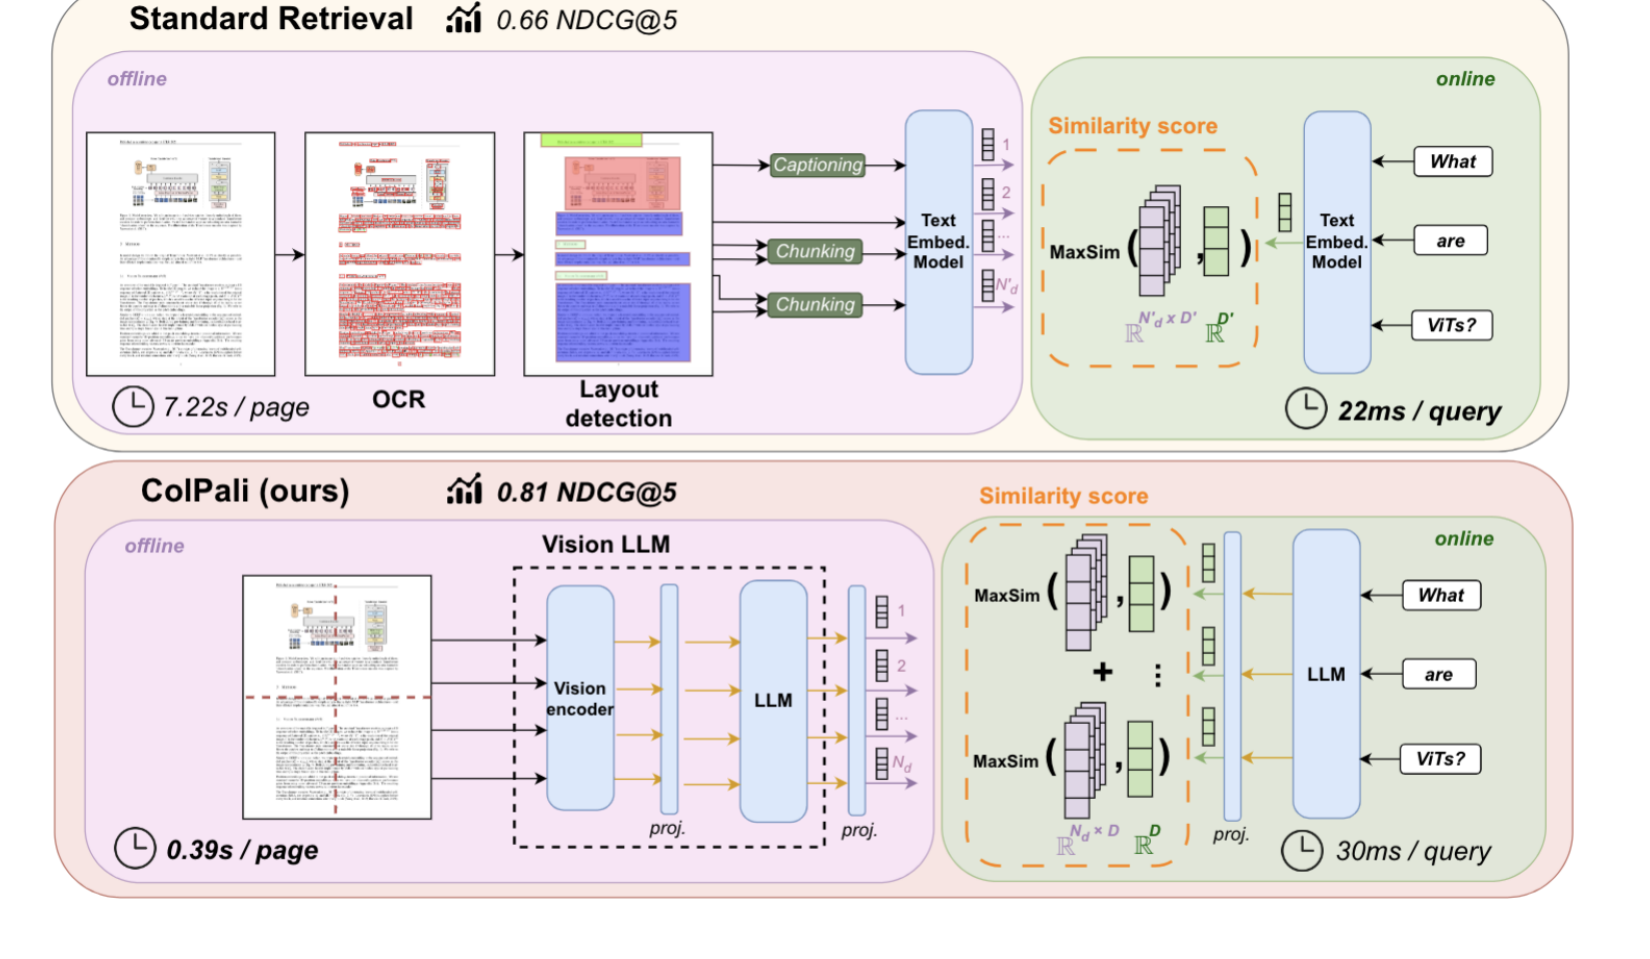
\includegraphics[width=\textwidth]{figures/tv2/colpali-pipeline.png}
    \caption[Quy trình truy xuất truyền thống và ColPali]{Lập chỉ mục và truy vấn ở pipeline truyền thống và ColPali. Nguồn: \cite{faysse2025colpali}.}
    \label{fig:tv2_colpali_pipeline}
\end{figure}

Hình~\ref{fig:tv2_colpali_pipeline} tách bước lập chỉ mục khỏi bước
tìm kiếm. Hệ thống mã hóa ảnh và lập chỉ mục trước khi có câu hỏi.
Khi nhận truy vấn, ColPali nối thêm năm token \texttt{<unused0>} rồi
mới mã hóa. Các token này giúp mô hình học cách mở rộng hoặc điều
chỉnh trọng số của truy vấn. Khi thêm trang mà vẫn dùng cùng mô hình
và quy tắc kết xuất, chỉ cần mã hóa phần mới. Nếu đổi checkpoint hoặc
độ phân giải, cần theo dõi phiên bản embedding để giữ chỉ mục nhất
quán \cite{faysse2025colpali,khattab2020colbert}.

\subsubsection{Toán tử Late Interaction (MaxSim) và hàm mất mát}

Với $\mathbf{q}_i$ là vector của token truy vấn thứ $i$ và $\mathbf{d}_j$
là vector thứ $j$ của trang, ColPali tính điểm theo cơ chế kế thừa từ
ColBERT \cite{khattab2020colbert,faysse2025colpali}
\begin{equation}
    \mathrm{LI}(q,d)
    = \sum_{i=1}^{N_q}\max_{1\le j\le N_d}
        \langle \mathbf{q}_i,\mathbf{d}_j\rangle.
\end{equation}
Mỗi token truy vấn đóng góp thông qua token trang khớp nhất. Do đó,
các từ khác nhau trong câu hỏi có thể khớp với các vùng ảnh khác nhau
trên cùng một trang.


\begin{examplebox}{Minh họa cách tính MaxSim}
Hai token truy vấn có điểm tương đồng với ba vùng của trang A lần lượt
là $(0{,}83,0{,}12,0{,}24)$ và $(0{,}28,0{,}66,0{,}34)$.
Điểm MaxSim của A là $0{,}83+0{,}66=1{,}49$. Trang B có một vùng
khớp token đầu ở mức $0{,}91$, nhưng token sau đạt tối đa $0{,}30$.
Điểm của B là $1{,}21$, nên A xếp trên B. Đây là ví dụ minh họa.
\end{examplebox}

Các token có thể khớp tại những vùng rời nhau. Tên một công ty có
thể nằm ở phần văn bản trong khi tỷ lệ tăng trưởng trên cùng trang
thuộc công ty khác. Điểm MaxSim cao giúp ưu tiên kiểm tra trang.
Bộ đọc còn phải xác minh số liệu thực sự gắn với công ty được hỏi.
Mỗi cặp truy vấn--trang cần $N_qN_d$ tích vô hướng trên vector $D$
chiều nếu chấm trực tiếp. Càng nhiều token hoặc ứng viên, MaxSim
càng phải tính nhiều. Khi đo trên kho lớn, cần ghi rõ số ứng viên
được chấm và cách nén vector.

\paragraph{Hard negatives trong ColPali.}
Với một batch gồm $B$ cặp $(q_i,d_i)$, ColPali dùng các trang của
những truy vấn khác làm in-batch negatives. Gọi $s_i^+$ là điểm của
trang liên quan và $s_i^-$ là điểm của negative được xếp cao nhất.
Hàm mất mát so sánh hai điểm như sau.
\begin{equation}
    \mathcal{L}_{\mathrm{ColPali}} =
    \frac{1}{B}\sum_{i=1}^{B}\log\bigl(1+\exp(s_i^- - s_i^+)\bigr).
    \label{eq:tv2_colpali_loss}
\end{equation}
Khi hard negative xếp trên trang liên quan, hiệu $s_i^- - s_i^+$
và mức phạt tăng. Nếu negative chứa một bản sao của cùng bảng, mô hình
có thể nhận tín hiệu phạt dù trang đó hữu ích. Cần xem xét
chất lượng nhãn khi áp dụng chiến lược này vào kho nhiều phiên bản
tài liệu.

Tập huấn luyện của ColPali chứa 118\,695 cặp truy vấn--trang. Khoảng
63\% đến từ dữ liệu học thuật công khai và 37\% là cặp tổng hợp từ
PDF. Nhóm tác giả dùng truy vấn tiếng Anh và kiểm tra để cùng một PDF
nhiều trang không xuất hiện trong cả tập huấn luyện lẫn tập đánh giá. Cấu hình tham chiếu
huấn luyện 1 epoch với LoRA ($r=32$, $\alpha=32$) ở phần ngôn ngữ,
cùng lớp chiếu mới khởi tạo. Bộ mã hóa ảnh được mở khóa trong một
thí nghiệm khác, xem kết quả ở Mục~\ref{subsec:tv2_ablation}
\cite{faysse2025colpali}.

\subsubsection{Đọc similarity heatmap của truy vấn}

Các điểm $\langle\mathbf{q}_i,\mathbf{d}_j\rangle$ của một token có
thể được đặt trở lại lưới ảnh. Hình~\ref{fig:tv2_colpali_heatmap}
cho thấy token \textit{hour} có điểm tương đồng nổi bật tại chữ
\textit{Hourly} và vùng trục hoành ghi giờ. Với ví dụ khác trong
phụ lục ColPali, từ khóa Kazakhstan còn kích hoạt vùng ghi
Kashagan, một mỏ dầu ở Kazakhstan \cite{faysse2025colpali}.

\begin{figure}[htbp]
    \centering
    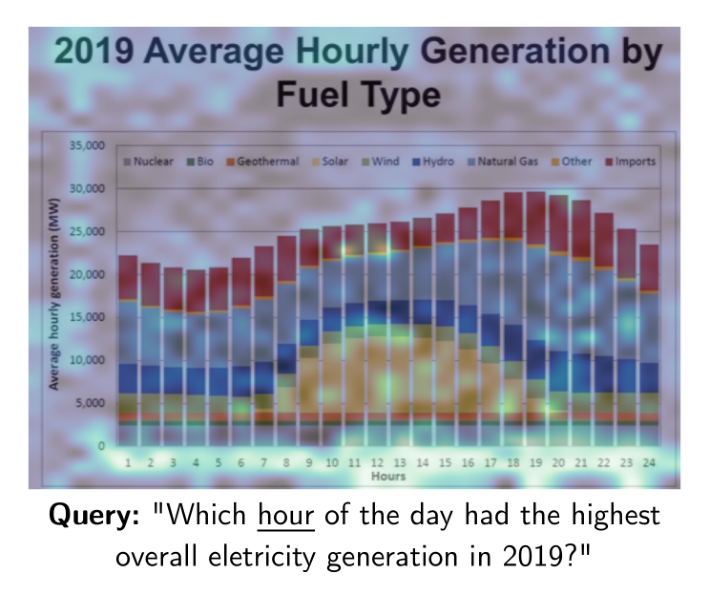
\includegraphics[width=0.72\textwidth]{figures/tv2/colpali-heatmap.png}
    \caption[Bản đồ tương đồng của token hour]{Tương đồng theo mảnh ảnh đối với token \textit{hour}. Nguồn: \cite{faysse2025colpali}.}
    \label{fig:tv2_colpali_heatmap}
\end{figure}

Các vùng sáng giải thích phần nào lý do trang nhận điểm truy xuất cao. Muốn trả lời giờ có tổng sản lượng lớn nhất, bộ đọc còn cần tìm cột cao nhất, xác định đúng số giờ trên trục và đọc phạm vi của biểu đồ. Heatmap hữu ích để kiểm tra chứng cứ mà retriever ưu tiên. Cần đối chiếu riêng nội dung trả lời do bộ sinh đưa ra.

\subsection{VisRAG với Single-vector Embeddings và End-to-End RAG}
\label{subsec:visrag}

\subsubsection{Bộ truy xuất VisRAG-Ret và Position-weighted Mean Pooling}

VisRAG-Ret dùng MiniCPM-V 2.0 để mã hóa câu hỏi và ảnh trang. Cho chuỗi
trạng thái ẩn $\mathbf{h}_1,\ldots,\mathbf{h}_n$, bộ truy xuất gộp chúng
thành một vector với trọng số tăng theo vị trí
\begin{equation}
    \mathbf{e}=\sum_{i=1}^{n}\frac{i}{\sum_{j=1}^{n}j}\,\mathbf{h}_i.
\end{equation}
Các token ở cuối chuỗi có thể tiếp nhận nhiều ngữ cảnh trước đó hơn
nhờ cơ chế causal attention. Điểm truy xuất là cosine similarity
giữa vector truy vấn và vector trang \cite{yu2025visrag}.


Với bốn vị trí, trọng số gộp lần lượt là $0{,}1$, $0{,}2$, $0{,}3$
và $0{,}4$. Hệ thống thu được một vector 2304 chiều cho mỗi trang.
Khi hai vector đã chuẩn hóa theo chuẩn Euclid, cosine tương đương
tích vô hướng. Chỉ mục vector có thể dùng Approximate Nearest
Neighbor (ANN) search. Đổi tham số tìm kiếm có thể giảm độ trễ nhưng cũng
loại trang liên quan khỏi danh sách ứng viên. Vì thế cần đo tỷ lệ
giữ lại trang đúng khi đánh giá tốc độ ở quy mô lớn.

Với truy vấn $q_i$, tập $D_i^-$ gồm các in-batch negatives,
còn $d_i^+$ là trang liên quan. InfoNCE có dạng
\begin{equation}
    \ell_i=-\log
    \frac{\exp(s(q_i,d_i^+)/\tau)}
    {\exp(s(q_i,d_i^+)/\tau)+
      \sum_{d\in D_i^-}\exp(s(q_i,d)/\tau)}.
    \label{eq:tv2_visrag_loss}
\end{equation}
Các negative có điểm cao đóng góp nhiều hơn trong mẫu số.
VisRAG huấn luyện 1 epoch với batch size 128 và $\tau=0{,}02$. Dữ liệu
kết hợp sáu tập hỏi đáp trực quan với các cặp tổng hợp từ giáo
trình, bài báo và tài liệu hướng dẫn. Một câu như “màu đường
thứ hai trong hình này là gì?” có thể được trả lời khi trang đã
cho sẵn, nhưng từ “hình này” ít giá trị trong tìm kiếm độc lập.
Bộ lọc loại các câu phụ thuộc mạnh vào trang cho trước để xây
dựng cặp phù hợp hơn cho huấn luyện truy xuất \cite{yu2025visrag}.

\subsubsection{Bộ tạo sinh VisRAG-Gen cho ngữ cảnh đa trang}
VisRAG-Gen khảo sát ba cách sử dụng các trang đã truy xuất. Với VLM
chỉ nhận một ảnh, hệ thống có thể ghép nhiều trang thành một ảnh
hoặc tạo câu trả lời riêng cho từng trang rồi chọn theo điểm kết hợp
độ tin cậy của bộ sinh với mức liên quan của trang. Với VLM hỗ trợ
nhiều ảnh, hệ thống đưa các trang riêng vào cùng một lượt suy luận
\cite{yu2025visrag}.

Hình~\ref{fig:tv2_visrag_pipeline} minh họa câu hỏi về sự thay đổi độ nhạy tần số từ đáy đến đỉnh ốc tai. Văn bản trích xuất chứa nhiều giá trị Hz rời rạc. Sơ đồ gốc giữ vị trí của từng nhãn số tương ứng cấu trúc giải phẫu, cho phép đọc được xu hướng giảm dần. Ví dụ cho thấy phần lớn ký tự vẫn có thể xuất hiện trong văn bản mà chứng cứ cần cho câu hỏi đã bị mất một phần \cite{yu2025visrag}.

\begin{figure}[htbp]
    \centering
    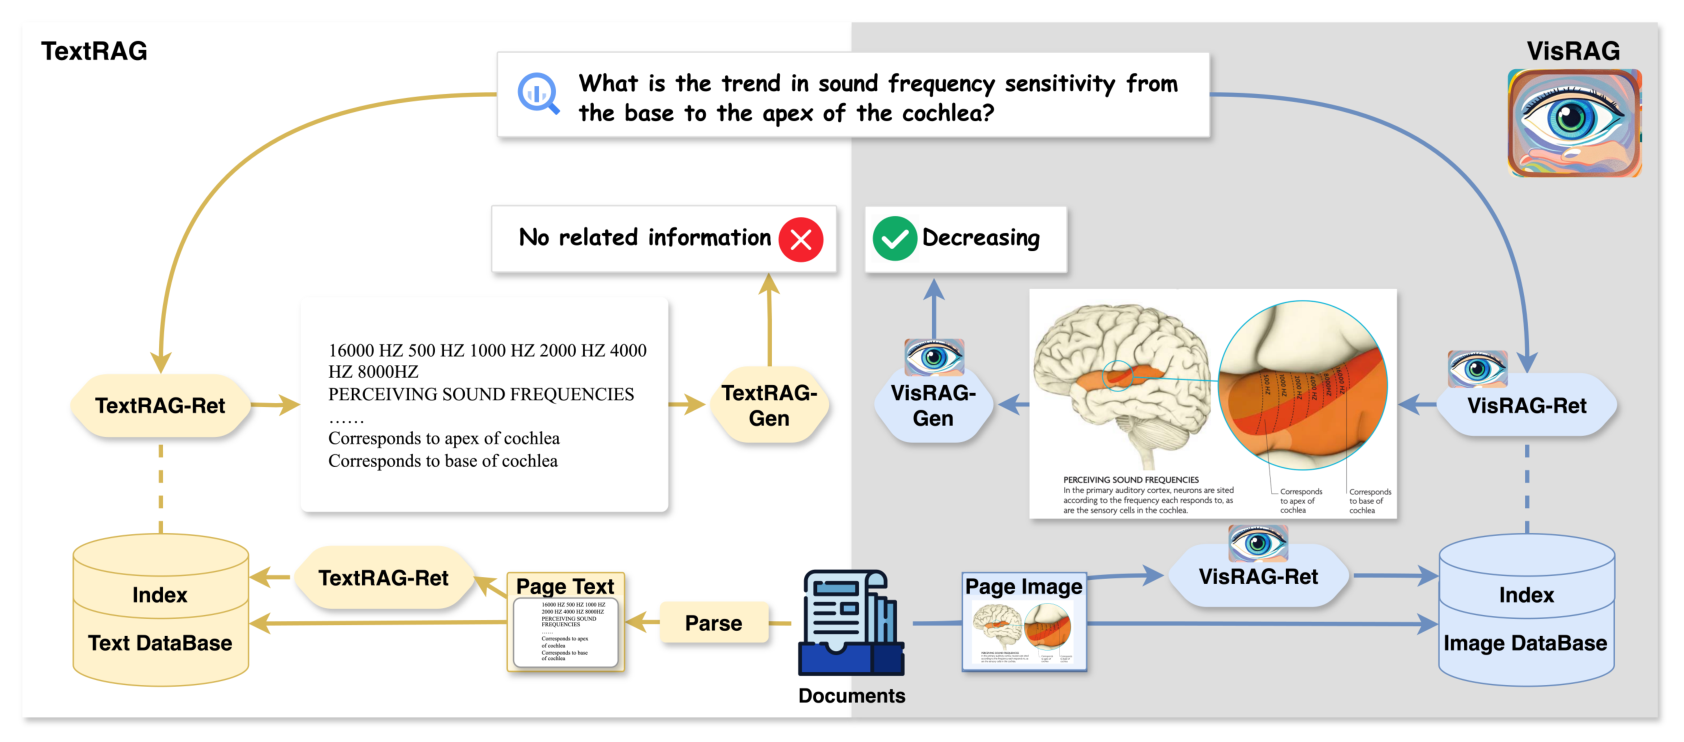
\includegraphics[width=\textwidth]{figures/tv2/visrag-pipeline.png}
    \caption[Luồng xử lý của TextRAG và VisRAG]{Luồng xử lý của TextRAG và VisRAG trong ví dụ sơ đồ ốc tai. Nguồn: \cite{yu2025visrag}.}
    \label{fig:tv2_visrag_pipeline}
\end{figure}

\paragraph{Page Concatenation.}
Các trang được ghép ngang thành một ảnh. MiniCPM-V~2.0 đọc ảnh ghép trong một lượt. Nếu ảnh ghép phải thu nhỏ, chữ nhỏ và các ô ở sát nhau khó phân biệt hơn. Cấu hình ghép còn đặt các trang liền kề dù chúng có thể nằm ở những phần khác nhau của tài liệu.

\paragraph{Weighted Selection.}
Mô hình tạo câu trả lời $a_d$ từ từng trang, sau đó chọn
theo điểm
\begin{equation}
    S(a_d,q,d)=g(a_d\mid q,d)
        \frac{\exp(s(q,d))}
        {\sum_{d'\in\mathcal{D}_{k}}\exp(s(q,d'))},
    \label{eq:tv2_visrag_selection}
\end{equation}
trong đó $\mathcal{D}_{k}$ là tập trang đã truy xuất và $g$ là độ
tin cậy tạo sinh, được tính bằng nghịch đảo perplexity trong bài
gốc. Mỗi câu trả lời ứng viên chỉ dùng một trang. Cấu hình này có
thể chọn được trang hữu ích khi thông tin nằm gọn trên một ảnh.
Nếu câu hỏi cần lấy số liệu từ hai trang, hai câu trả lời riêng
có thể đều thiếu một phần chứng cứ \cite{yu2025visrag}.

\paragraph{Multi-image VLM.}
MiniCPM-V 2.6 và GPT-4o có thể nhận từng ảnh trong cùng một lượt.
Ví dụ, một trang chứa bảng doanh thu và trang kế tiếp ghi đơn
vị quy đổi. Đưa cả hai ảnh vào cho phép đối chiếu giá trị với đơn
vị trước khi tính. Số ảnh tăng cũng làm tăng số token thị giác,
độ trễ và khả năng có trang nhiễu. Thực nghiệm ở
Mục~\ref{subsec:tv2_generation} phân tích kết quả theo số trang
và theo năng lực xử lý ảnh của từng bộ sinh.

\subsubsection{Hai loại lỗi quan sát trên bài kiểm thử}

Trong ví dụ Club Jetty ở Bảng 8 của VisRAG, OCR đọc sai tên nhà
hàng do chữ cách điệu. TextRAG lấy nhầm trang Smokers Express.
VisRAG trả đúng trang \textit{Explore Kauai}, nơi ô quảng cáo ghi
nhà hàng đóng cửa thứ Ba. Đây là lỗi truy xuất. Khi cửa hàng cần
hỏi không xuất hiện trong ngữ cảnh, tăng năng lực bộ sinh khó
khôi phục chứng cứ bị thiếu \cite{yu2025visrag}.

Trong ví dụ LinkedIn ở Bảng 9, cả hai cấu hình đều tìm đúng
infographic. TextRAG trả 49\%, tỷ lệ của Bắc Mỹ, dù truy vấn hỏi
về châu Âu. VisRAG đọc đúng 53\% từ vị trí của nhãn châu Âu.
Lỗi xảy ra sau khi đã tìm đúng trang, ở bước chuẩn bị hoặc đọc
ngữ cảnh. Cả hai phương án đều tìm đúng trang ở hạng đầu nên có cùng
Recall@1 cho câu hỏi này, dù đáp án khác nhau \cite{yu2025visrag}.

\subsection{So sánh đối chứng chuyên sâu: ColPali và VisRAG}
\label{subsec:colpali_vs_visrag}


\begin{table}[H]
\centering
\small
\caption[Bảng đối chứng cơ chế kỹ thuật giữa ColPali và VisRAG]{Bảng đối chứng cơ chế kỹ thuật và đánh đổi thiết kế giữa ColPali và VisRAG.}
\label{tab:colpali_vs_visrag}
\renewcommand{\arraystretch}{1.24}
\begin{tabularx}{\textwidth}{@{}P{3.4cm}L L@{}}
\toprule
\rowcolor{tblhead}
\thead{Tiêu chí đối chiếu} & \thead{ColPali} & \thead{VisRAG} \\
\midrule
Backbone nền tảng & PaliGemma-3B & MiniCPM-V 2.0 (bộ truy xuất) \\
\rowcolor{zebrabg}
Kiểu biểu diễn \& Dung lượng & 1030 vector 128 chiều, khoảng 257,5\,KB/trang & Một vector 2304 chiều, khoảng 4,5\,KB/trang \\
Cơ chế so khớp & Tổng MaxSim theo token & Cosine giữa hai vector gộp \\
\rowcolor{zebrabg}
Khả năng giải thích & Có thể minh họa vùng ảnh khớp với token & Điểm tương đồng ở mức toàn trang \\
Phạm vi giải quyết & Xếp hạng trang & Xếp hạng trang và tạo câu trả lời \\
\rowcolor{zebrabg}
Dữ liệu \& Huấn luyện & Cặp truy vấn--trang, mẫu âm trong batch & Dữ liệu VQA và cặp tổng hợp, mẫu âm trong batch \\
Điểm yếu / Đánh đổi chính & Chỉ mục lớn, nhiều phép so khớp khi chấm điểm & Gộp tín hiệu toàn trang vào một vector \\
\bottomrule
\end{tabularx}
\end{table}

Dung lượng trong Bảng~\ref{tab:colpali_vs_visrag} là kích thước biểu
diễn trang tương ứng với cấu hình của từng bài \cite{faysse2025colpali,yu2025visrag}. Biểu diễn
đa vector giữ tín hiệu ở nhiều vùng của trang. Biểu diễn đơn vector
cần ít bộ nhớ hơn và chấm điểm bằng cosine similarity.

Với hai byte cho mỗi giá trị, ColPali cần
$1030\times128\times2=263\,680$ byte mỗi trang, tương đương
257,5\,KiB. Vector 2304 chiều cần 4608 byte, tức 4,5\,KiB.
Bảng giữ ký hiệu KB theo hai nghiên cứu. Chênh lệch khoảng
57,2 lần áp dụng cho biểu diễn chưa nén. Với một triệu trang,
hai mức này lần lượt xấp xỉ 245,6\,GiB và 4,3\,GiB trước khi
tính cấu trúc chỉ mục, metadata, ảnh tài liệu và bộ nhớ mô hình.
Các lựa chọn độ chính xác lưu trữ khác làm thay đổi dự toán
\cite{faysse2025colpali,yu2025visrag}.

Trên kho báo cáo dày chữ, cần kiểm tra khả năng giữ đúng trang
có bảng và khả năng nén chỉ mục mà không mất vùng chữ nhỏ. Trên
kho lớn và đa dạng, chỉ mục vector đơn thuận tiện để thử tìm kiếm
ứng viên. Các kết quả theo từng tập ở Mục~\ref{subsec:tv2_visrag_ret_results}
cho thấy thứ hạng của hai phương pháp thay đổi giữa DocVQA, SlideVQA,
InfoVQA và PlotQA. Vì vậy, phép đánh giá nên phản ánh loại câu hỏi
người dùng thường gặp, như tìm mã định danh, đọc bảng hay giải thích
biểu đồ.

Có thể dùng vector đơn chọn $m$ ứng viên rồi dùng MaxSim xếp hạng lại. Khi đó cần lưu thêm vector hoặc mã hóa lại ảnh ứng viên. Recall của top-$m$ là giới hạn của bước xếp hạng lại. Mục~\ref{subsec:tv2_protocol} đề xuất cách đo khi kết hợp hai tầng.
% ==============================================================================
% Section 3.3: Post-Retrieval Knowledge Reconciliation - CoRe-MMRAG (Clean Skeleton)
% Owner: Member 3 (TV3) | Target length: ~3-3.5 pages
% ==============================================================================

\section{Tầng Post-Retrieval: Hòa giải xung đột tri thức đa nguồn -- CoRe-MMRAG}
\label{sec:method_coremmrag}

\draftnote[TV3]{QUAN TRỌNG: Ghi chú trong Google Docs về bài 5 còn sơ lược và thiếu số liệu. TV3 cần đọc trực tiếp bản PDF gốc \textit{CoRe-MMRAG} (\texttt{2025.acl-long.1583}, \texttt{\textbackslash cite\{tian2025coremmrag\}}) để viết đầy đủ mục này với độ dài 3--3.5 trang.}

\subsection{Hình thức hóa xung đột tri thức trong Multimodal RAG: PRKI và VTKI}
\label{subsec:core_conflicts}

\draftnote[TV3]{Định nghĩa và phân biệt rõ 2 dạng xung đột cốt lõi của bài báo: (1) PRKI (\textit{Parametric-Retrieved Knowledge Inconsistency} -- mâu thuẫn giữa tri thức tham số nội tại và dữ liệu truy xuất ngoài); (2) VTKI (\textit{Visual-Textual Knowledge Inconsistency} -- mâu thuẫn giữa tín hiệu thị giác trong ảnh và văn bản truy xuất). Kèm 1 ví dụ minh họa cụ thể từ bài gốc.}

\subsection{Cơ chế hoạt động 4 giai đoạn của CoRe-MMRAG}
\label{subsec:core_pipeline}

\draftnote[TV3]{Vẽ/chèn sơ đồ pipeline và giải thích chi tiết từng bước trong quy trình 4 giai đoạn: (1) Parametric Knowledge Generation; (2) Visual-Textual Knowledge Integration (đánh giá tương đồng liên hợp để lọc nhiễu VTKI); (3) External Response Generation; (4) Cross-Source Integration \& Reconciliation (hòa giải PRKI). Bổ sung công thức tương ứng từ PDF gốc.}

\subsection{Mô hình huấn luyện chuyên biệt và đánh đổi suy luận}
\label{subsec:core_training}

\draftnote[TV3]{Trình bày chiến lược huấn luyện phân biệt nguồn tri thức và căn chỉnh đa phương thức từ bài gốc; phân tích 2 đánh đổi: (1) tăng chi phí suy luận và độ trễ (Inference Overhead) do chạy chuỗi nhiều bước; (2) hiệu năng bị chặn trần bởi năng lực nhận thức chi tiết ảnh của MLLM nền.}

% ==============================================================================
% Section 3.4: Cross-Method Comparison and Unified Architecture (Clean Skeleton)
% Owner: Member 3 (TV3) | Target length: ~2 pages
% ==============================================================================

\section{Tổng hợp mối liên hệ, độ phức tạp và khả năng kết hợp}
\label{sec:method_integration}

\draftnote[TV3]{Mục 3.4 dài khoảng 2 trang. Đây là mục tổng hợp liên kết toàn bộ 4 phương pháp kỹ thuật theo khía cạnh: độ phức tạp, phạm vi giải quyết, khả năng ghép nối thành một kiến trúc đầu--cuối và các điểm nghẽn khi tích hợp.}

\subsection{Ma trận so sánh toàn diện bốn phương pháp}
\label{subsec:4method_matrix}

\draftnote[TV3]{Hoàn thiện Bảng~\ref{tab:four_methods_summary} đối chiếu UniversalRAG, ColPali, VisRAG và CoRe-MMRAG theo các trục: Tầng xử lý, Bài toán giải quyết, Chi phí/Độ phức tạp (thời gian, bộ nhớ) và Điều kiện thất bại.}

\begin{table}[H]
\centering
\small
\caption[So sánh tổng hợp 4 phương pháp trọng tâm]{So sánh tổng hợp 4 phương pháp trọng tâm theo tầng xử lý, phạm vi và độ phức tạp.}
\label{tab:four_methods_summary}
\renewcommand{\arraystretch}{1.24}
\begin{tabularx}{\textwidth}{@{}P{3.0cm}P{2.3cm}L L P{2.7cm}@{}}
\toprule
\rowcolor{tblhead}
\thead{Phương pháp} & \thead{Tầng xử lý} & \thead{Bài toán giải quyết} & \thead{Chi phí / Độ phức tạp} & \thead{Điều kiện thất bại} \\
\midrule
UniversalRAG & \dots & \dots & \dots & \dots \\
\rowcolor{zebrabg}
ColPali & \dots & \dots & \dots & \dots \\
VisRAG & \dots & \dots & \dots & \dots \\
\rowcolor{zebrabg}
CoRe-MMRAG & \dots & \dots & \dots & \dots \\
\bottomrule
\end{tabularx}
\end{table}

\subsection{Kiến trúc tích hợp đề xuất và các điểm nghẽn khi kết hợp}
\label{subsec:unified_architecture}

\draftnote[TV3]{Đề xuất kịch bản ghép nối cả 4 phương pháp thành một pipeline tham chiếu thống nhất (UniversalRAG định tuyến $\rightarrow$ ColPali/VisRAG xử lý kho tài liệu trực quan $\rightarrow$ CoRe-MMRAG hòa giải xung đột PRKI/VTKI $\rightarrow$ tạo sinh câu trả lời). Có thể đặt nhận định cốt lõi vào môi trường \texttt{keybox}. Phân tích 3 điểm nghẽn thực tế khi tích hợp: cộng dồn độ trễ, lan truyền sai số xuyên tầng (cascading errors) và chi phí đồng bộ nhiều mô hình nền khác nhau.}


% ==============================================================================
% Chapter 4: Datasets, Evaluation Metrics, and Experimental Analysis (Clean Skeleton)
% Owners: TV1 (UniversalRAG), TV2 (ColPali & VisRAG), TV3 (Comparability & CoRe-MMRAG)
% Target length: ~7-9 pages
% ==============================================================================

\chapter{Dữ liệu, độ đo và phân tích kết quả thực nghiệm}
\label{chap:experiments}

\draftnote[Chung]{Chương 4 dài khoảng 7--9 trang. Không chép máy móc bảng số liệu thô: phải làm rõ điều kiện đánh giá, trả lời trực diện câu hỏi "các kết quả có so sánh trực tiếp được không?", và kiểm chứng xem thực nghiệm có thực sự chứng minh được tuyên bố của tác giả hay không.}

% ------------------------------------------------------------------------------
\section{Tổng quan bộ dữ liệu và benchmark đánh giá}
\label{sec:exp_datasets}

\draftnote[TV1 + TV2 + TV3]{Mỗi thành viên điền và phân tích nhóm benchmark thuộc phần mình phụ trách vào Bảng~\ref{tab:benchmarks}: ViDoRe 10 tác vụ Anh--Pháp (ColPali); 6 tập VQA + BEIR (VisRAG); 10 tập ID + 6 tập OOD (UniversalRAG); InfoSeek \& Encyclopedic-VQA (CoRe-MMRAG). Nêu rõ đặc điểm thống kê cơ bản cần thiết để hiểu và đối chiếu kết quả.}

\begin{table}[H]
\centering
\small
\caption[Tổng hợp các bộ dữ liệu và benchmark trọng tâm]{Tổng hợp các bộ dữ liệu và benchmark trọng tâm được sử dụng trong 4 nghiên cứu kỹ thuật.}
\label{tab:benchmarks}
\renewcommand{\arraystretch}{1.24}
\begin{tabularx}{\textwidth}{@{}P{3.1cm}P{2.5cm}P{2.3cm}L@{}}
\toprule
\rowcolor{tblhead}
\thead{Nhóm / Benchmark} & \thead{Bài báo} & \thead{Phương thức} & \thead{Đặc điểm nổi bật \& Thách thức} \\
\midrule
ViDoRe & ColPali & \dots & \dots \\
\rowcolor{zebrabg}
6 tập VQA + BEIR & VisRAG & \dots & \dots \\
10 tập ID + 6 tập OOD & UniversalRAG & Văn bản, bảng, ảnh, video & 7 lựa chọn định tuyến theo phương thức và mức độ chi tiết (10 tập ID chia 3:7; 6 tập OOD chỉ dùng kiểm thử); đánh giá cả truy xuất đơn kho và liên phương thức \cite{yeo2026universalrag} \\
\rowcolor{zebrabg}
InfoSeek \& Enc-VQA & CoRe-MMRAG & \dots & \dots \\
\bottomrule
\end{tabularx}
\end{table}

% TV1: Dataset and evaluation protocol breakdown for UniversalRAG
\paragraph{Hệ thống 16 bộ dữ liệu đa phương thức và nhiều mức độ chi tiết của UniversalRAG.}
Để đánh giá khả năng chọn đồng thời phương thức và mức độ chi tiết, UniversalRAG \cite{yeo2026universalrag} sử dụng 10 bộ dữ liệu cùng phân phối (\textit{in-domain} -- ID) và 6 bộ dữ liệu khác phân phối (\textit{out-of-domain} -- OOD) (Bảng~7 và Phụ lục~A của bài gốc). Mười tập ID được chia theo tỷ lệ 3:7 để huấn luyện bộ định tuyến và kiểm thử, bao phủ đủ 7 lựa chọn định tuyến:
\begin{itemize}
    \item \textit{Không cần truy xuất (None)}: MMLU gồm 1\,710 câu hỏi trắc nghiệm lấy từ tập \textit{dev}, dùng để kiểm tra xem hệ thống có tránh được bước truy xuất không cần thiết khi câu hỏi chỉ cần kiến thức phổ thông hay không.
    \item \textit{Văn bản ở hai mức độ chi tiết (Paragraph và Document)}: Natural Questions (NQ) gồm 2\,000 câu hỏi tra cứu một bước trên kho 850k đoạn Wikipedia (tối đa 100 từ, trung bình 100 token). HotpotQA gồm 2\,000 câu hỏi suy luận nhiều bước trên kho 509k tài liệu gộp liên quan (trung bình 693 token, nhiều mẫu dài trên 4k token theo cách ghép của LongRAG).
    \item \textit{Kết hợp văn bản và bảng (Paragraph+Table)}: HybridQA gồm 2\,000 câu hỏi với kho 15k mục. Khác với bản gốc vốn nối sẵn bảng Wikipedia với đoạn văn liên quan, nhóm tác giả tách chúng thành hai kho riêng để kiểm tra khả năng gọi đồng thời cả hai kho.
    \item \textit{Ảnh và kết hợp văn bản với ảnh}: MRAG-Bench gồm 1\,353 câu hỏi có kèm ảnh đầu vào trên kho 6k ảnh. WebQA gồm 2\,000 câu hỏi văn bản (đã lọc qua GPT-4o để bỏ các câu gắn cứng với một bức ảnh duy nhất) trên kho 20k đoạn văn và ảnh tách rời. InfoSeek gồm 2\,000 câu hỏi văn bản kèm ảnh từ tập \textit{dev} trên kho 20k đoạn văn và ảnh.
    \item \textit{Video ở hai mức độ chi tiết (Clip và Video)}: LVBench gồm 777 câu hỏi trên 89 video YouTube dài trung bình 3\,865 giây; phần lớn câu hỏi có mốc thời gian đáp án ngắn hơn 5 phút nên được xếp vào nhóm cần đoạn ngắn (Clip). Hai tập VideoRAG-Wiki và VideoRAG-Synth có 374 câu hỏi mỗi tập, dùng chung kho 9k video hướng dẫn HowTo100M dài trung bình 378 giây và đại diện cho nhóm cần xem toàn bộ video (Video).
\end{itemize}

Sáu tập OOD chỉ dùng ở bước kiểm thử mà không đưa vào huấn luyện bộ định tuyến, gồm: TruthfulQA (None, 790 câu trắc nghiệm), TriviaQA (Paragraph, 661 câu, kho 661k đoạn), SQuAD~v1.1 (Paragraph, 2\,000 câu, kho 1,19 triệu đoạn Wikipedia), 2WikiMultiHopQA (Document, 2\,000 câu, kho 12k tài liệu dài trung bình 562 token), Visual-RAG (Image, 374 câu hỏi văn bản tìm ảnh, kho 2k ảnh) và CinePile (Clip/Video, 1\,440 câu hỏi trên 144 video dài trung bình 158 giây).

Khi đọc số liệu của bài báo (Phụ lục~A.1--A.3 của \cite{yeo2026universalrag}), cần lưu ý hai chi tiết về cách chuẩn bị dữ liệu và tính điểm. Thứ nhất, hai tập LVBench và CinePile vốn là dữ liệu hỏi đáp trên một video cho sẵn chứ không phải bài toán tìm kiếm mở, nên nhóm tác giả đã dùng GPT-4o viết lại câu hỏi sang dạng văn bản độc lập dựa trên tiêu đề và thông tin kênh YouTube. Việc tách nhãn Clip/Video trên VideoRAG, CinePile cũng như bước lọc câu hỏi trên TriviaQA, WebQA đều do GPT-4o thực hiện. Thứ hai, mỗi nhóm tác vụ dùng độ đo riêng: \textit{Top-1 Accuracy} cho câu trắc nghiệm (MMLU, MRAG-Bench, LVBench, TruthfulQA, CinePile), \textit{Exact Match} (EM) và F1 cho câu trả lời ngắn (NQ, HotpotQA, HybridQA, TriviaQA, SQuAD, 2WikiMultiHopQA), độ chính xác theo quy ước gốc cho InfoSeek, và \textit{ROUGE-L} cùng \textit{BERTScore} cho câu trả lời dài tự do (WebQA, VideoRAG-Wiki/Synth, Visual-RAG). Điểm trung bình chung (Avg) được tính bằng cách lấy trung bình trong từng phương thức trước rồi mới lấy trung bình giữa các phương thức để các tập văn bản không chiếm trọng số quá lớn. Ngoài ra, toàn bộ kết quả được lấy từ một lần chạy duy nhất (\textit{single run}).

% ------------------------------------------------------------------------------
\section{Hệ thống độ đo đánh giá}
\label{sec:exp_metrics}

\draftnote[TV2]{Trình bày ngắn gọn định nghĩa, công thức chính và ý nghĩa khác biệt của 3 nhóm độ đo: (1) Truy xuất ($\mathrm{MRR}@K$, $\mathrm{nDCG}@K$, $\mathrm{Recall}@K$); (2) Tạo sinh \& Định tuyến ($\mathrm{EM}$, $\mathrm{Relaxed\ EM\ (\pm 5\%)}$, $\mathrm{VQA\ Accuracy}$, $\mathrm{BEM}$, $\mathrm{Routing\ Accuracy}$); (3) Hiệu năng hệ thống (Offline Indexing Latency, Online Query Latency, Storage Footprint KB/page).}

% ------------------------------------------------------------------------------
\section{Phân tích tính khả so sánh và đối chiếu kết quả định lượng}
\label{sec:exp_results}

\subsection{Các kết quả có thể so sánh trực tiếp không?}
\label{subsec:comparability}

\draftnote[TV3]{Trả lời trực tiếp yêu cầu bài tập: (1) Chỉ có cặp \textbf{ColPali và VisRAG} đối chiếu trực tiếp được trên phân khúc truy xuất tài liệu trực quan (VisRAG báo cáo trực tiếp In-domain MRR@10 cùng đối chiếu tốc độ và bộ nhớ); (2) Không so sánh ngang hàng bằng 1 con số duy nhất giữa UniversalRAG, CoRe-MMRAG và ColPali/VisRAG do khác bộ dữ liệu, đơn vị truy xuất, backbone và độ đo; (3) Lưu ý điểm giao tập \texttt{InfoSeek} giữa UniversalRAG và CoRe-MMRAG khác thiết lập nên phải phân tích riêng điều kiện thực nghiệm.}

\subsection{Tổng hợp kết quả định lượng theo từng nhóm bài toán}
\label{subsec:quantitative_tables}

\draftnote[TV2]{Điền Bảng~\ref{tab:vision_vs_text_retrieval} (đối chiếu Vision-space ColPali, ColQwen2, VisRAG-Ret với TextRAG OCR/Captioning, SigLIP, BiPali, ColSigLIP kèm trích nguồn Bảng/Hình bài gốc). Đồng thời bổ sung thêm 1 bảng hoặc mục phân tích nhỏ cho: (a) End-to-End Generation của VisRAG (MiniCPM-V 2.6, GPT-4o, top-1/3/6/10, BEIR); (b) Ablation Study của ColPali (448 vs 224, OOD DocMatix, bỏ \texttt{<unused0>}, Token Pooling factor=3).}

\begin{table}[H]
\centering
\small
\caption[Đối chiếu hiệu năng truy xuất, tốc độ và dung lượng giữa Vision-space RAG và TextRAG]{Đối chiếu hiệu năng truy xuất, tốc độ và dung lượng lưu trữ giữa Vision-space RAG và TextRAG.}
\label{tab:vision_vs_text_retrieval}
\renewcommand{\arraystretch}{1.24}
\begin{tabularx}{\textwidth}{@{}L M{2.05cm} M{2.15cm} M{1.75cm} M{2.05cm}@{}}
\toprule
\rowcolor{tblhead}
\thead{Phương pháp} & \thead{ViDoRe\newline (nDCG@5)} & \thead{VisRAG ID\newline (MRR@10)} & \thead{Index /\newline trang} & \thead{Dung lượng /\newline trang} \\
\midrule
Baseline TextRAG / VLM & \dots & \dots & \dots & \dots \\
\rowcolor{zebrabg}
ColPali / ColQwen2 & \dots & \dots & \dots & \dots \\
VisRAG-Ret & \dots & \dots & \dots & \dots \\
\bottomrule
\end{tabularx}
\end{table}

% TV1: Quantitative analysis for UniversalRAG
\subsubsection{Kết quả định lượng của UniversalRAG trên các tập ID và OOD}
\label{subsubsec:universalrag_quant}

UniversalRAG được so sánh với 12 phương pháp cơ sở chia thành 4 nhóm (Mục~3.1 của \cite{yeo2026universalrag}): trả lời trực tiếp không truy xuất (Naïve), 6 hệ thống RAG cố định một kho đơn lẻ (ParagraphRAG, DocumentRAG, TableRAG, ImageRAG, ClipRAG, VideoRAG), 4 phương pháp đưa mọi dữ liệu vào chung một không gian vector (UniRAG, GME, $\mathrm{PE}_{\mathrm{core}}$, VLM2Vec-V2) và phương pháp lấy ngữ cảnh từ tất cả các kho cùng lúc (MultiRAG). Bảng~\ref{tab:universalrag_results} tổng hợp kết quả tạo sinh trên 10 tập ID khi dùng mô hình sinh Qwen3-VL-8B-Instruct.

\begin{table}[H]
\centering
\footnotesize
\caption[Kết quả tạo sinh của UniversalRAG trên 10 tập In-Domain]{Kết quả tạo sinh của UniversalRAG và các phương pháp đối chứng trên 10 tập In-Domain với mô hình sinh Qwen3-VL-8B-Instruct (Nguồn: Bảng~1 của \cite{yeo2026universalrag}). Cột Avg tính trung bình theo từng phương thức (đã tính cả VideoRAG-Wiki: Naïve 19,78; Qwen3-VL-2B 20,86; Oracle 20,89 theo ROUGE-L).}
\label{tab:universalrag_results}
\setlength{\tabcolsep}{2.7pt}
\renewcommand{\arraystretch}{1.18}
\begin{tabularx}{\textwidth}{@{}L *{10}{r}@{}}
\toprule
\rowcolor{tblhead}
\thead{Phương pháp} & \thead{MMLU} & \thead{NQ} & \thead{Hotpot} & \thead{Hybrid} & \thead{MRAG} & \thead{WebQA} & \thead{InfoS.} & \thead{LVB} & \thead{Vid-S} & \thead{Avg} \\
\rowcolor{tblhead}
 & \scriptsize{(Acc)} & \scriptsize{(EM)} & \scriptsize{(EM)} & \scriptsize{(EM)} & \scriptsize{(Acc)} & \scriptsize{(R-L)} & \scriptsize{(Acc)} & \scriptsize{(Acc)} & \scriptsize{(R-L)} & \\
\midrule
Naïve (Không truy xuất) & 74,39 & 18,85 & 21,10 & 2,80 & 49,22 & 58,12 & 18,10 & 28,83 & 35,86 & 35,59 \\
\midrule
\rowcolor{zebrabg}
ParagraphRAG & 74,39 & 39,25 & 23,40 & 5,10 & 46,71 & 51,70 & 19,75 & 24,07 & 32,86 & 37,26 \\
DocumentRAG & 71,29 & 21,95 & 26,35 & 3,75 & 43,68 & 45,57 & 16,80 & 15,70 & 31,18 & 32,26 \\
\rowcolor{zebrabg}
TableRAG & 72,51 & 11,80 & 16,45 & 9,65 & 43,39 & 44,75 & 9,15 & 16,47 & 30,67 & 29,45 \\
ImageRAG & 73,33 & 17,15 & 19,15 & 2,20 & 52,55 & 67,96 & 20,15 & 25,35 & 36,10 & 35,04 \\
\rowcolor{zebrabg}
ClipRAG & 73,33 & 16,70 & 19,30 & 2,35 & 48,93 & 65,68 & 9,85 & 33,72 & 39,39 & 35,18 \\
VideoRAG & 74,91 & 15,85 & 20,00 & 2,30 & 48,04 & 64,97 & 11,25 & 32,05 & 40,05 & 35,01 \\
\midrule
\rowcolor{zebrabg}
UniRAG (Unified) & 70,06 & 19,30 & 19,35 & 2,85 & 44,86 & 53,26 & 19,05 & 22,65 & 32,41 & 32,93 \\
GME (Unified) & 70,41 & 20,05 & 19,50 & 3,00 & 49,45 & 55,03 & 19,20 & 23,68 & 33,02 & 33,88 \\
\rowcolor{zebrabg}
$\mathrm{PE}_{\mathrm{core}}$ (Unified) & 72,11 & 19,65 & 19,00 & 3,05 & 49,15 & 54,79 & 19,10 & 23,04 & 32,75 & 33,86 \\
VLM2Vec-V2 (Unified) & 71,70 & 19,95 & 18,50 & 2,95 & 46,78 & 52,35 & 18,80 & 23,55 & 33,38 & 33,31 \\
\rowcolor{zebrabg}
MultiRAG (All corpora) & 70,82 & 20,90 & 22,65 & 4,35 & 45,01 & 56,73 & 19,05 & 23,55 & 34,24 & 34,07 \\
\midrule
URAG (Qwen3-VL-2B) & 74,39 & 38,65 & \textbf{26,10} & \textbf{11,05} & \textbf{52,55} & \textbf{70,22} & 23,20 & \textbf{33,72} & \textbf{39,95} & \textbf{42,40} \\
\rowcolor{zebrabg}
URAG (InternVL3.5-1B) & 74,39 & \textbf{38,70} & 25,85 & 10,25 & \textbf{52,55} & 69,14 & \textbf{23,35} & \textbf{33,72} & 39,90 & 42,12 \\
URAG (T5Gemma 2 270M) & \textbf{74,62} & 38,65 & 25,90 & 9,95 & 50,33 & 69,03 & 21,95 & 33,59 & 39,43 & 41,68 \\
\rowcolor{zebrabg}
URAG (GPT-5, \textit{free}) & 74,27 & 34,50 & 24,35 & 4,95 & 50,11 & 62,38 & 21,45 & 32,30 & 35,94 & 39,26 \\
URAG (Qwen3-VL-8B, \textit{free}) & 74,09 & 35,20 & 24,65 & 5,25 & 50,04 & 65,27 & 20,65 & 32,43 & 34,77 & 39,46 \\
\midrule
\rowcolor{zebrabg}
Oracle (Cận trên) & 74,39 & 39,25 & 26,35 & 10,55 & 52,55 & 71,17 & 23,35 & 33,72 & 40,05 & 42,45 \\
\bottomrule
\end{tabularx}
\end{table}

Từ Bảng~\ref{tab:universalrag_results} có thể rút ra bốn nhận xét chính. Thứ nhất, các hệ thống RAG cố định một kho chỉ đạt kết quả tốt trên đúng tập dữ liệu khớp với phương thức và mức độ chi tiết của kho đó (ParagraphRAG đạt 39,25 EM trên NQ; DocumentRAG đạt 26,35 EM trên HotpotQA; ClipRAG đạt 33,72 Acc trên LVBench). Khi sang các tập khác loại, kết quả giảm mạnh do ngữ cảnh đưa vào không liên quan: ví dụ trên LVBench, ParagraphRAG chỉ đạt 24,07 so với 28,83 khi không truy xuất (Naïve), còn TableRAG kéo điểm trung bình chung xuống còn 29,45. Thứ hai, cả bốn phương pháp dùng chung không gian vector (UniRAG 32,93; GME 33,88; $\mathrm{PE}_{\mathrm{core}}$ 33,86; VLM2Vec-V2 33,31) lẫn MultiRAG (34,07) đều có điểm trung bình \textit{thấp hơn} cả mức không truy xuất Naïve (35,59). Điều này cho thấy việc lấy nhầm văn bản do khoảng cách phương thức hoặc nhồi cùng lúc dữ liệu từ mọi kho đều gây nhiễu cho mô hình sinh. Thứ ba, các biến thể bộ định tuyến có huấn luyện của UniversalRAG tiến rất sát cận trên Oracle (42,40 so với 42,45 ở Qwen3-VL-2B; biến thể nhỏ T5Gemma~2 270M cũng đạt 41,68). Riêng trên HybridQA, Qwen3-VL-2B đạt 11,05 EM, cao hơn nhẹ so với Oracle gán cứng theo tập (10,55 EM) nhờ bỏ bớt được nguồn không cần thiết ở một số câu hỏi đơn lẻ. Thứ tư, kết quả này lặp lại nhất quán trên hai mô hình sinh LVLM khác (Bảng~8 của \cite{yeo2026universalrag}): với InternVL3.5-8B, UniversalRAG (Qwen3-VL-2B) đạt trung bình 39,60 (so với Oracle 39,80, mức đơn kho cao nhất là ImageRAG 32,29, Naïve 31,29 và nhóm không gian vector chung 28,38--28,60); với Molmo2-4B, điểm đạt 41,83 (so với Oracle 42,05, ParagraphRAG 36,52, Naïve 33,19 và nhóm không gian vector chung 32,04--32,50).

\paragraph{Đánh giá vai trò của định tuyến phương thức, truy xuất liên phương thức và mức độ chi tiết.}
Bảng~\ref{tab:universalrag_routing_recall} trích dẫn độ chính xác chọn nhóm phương thức (\textit{Modality Accuracy} tính trên 4 nhóm lớn) cùng độ phủ truy xuất (\textit{Recall}@1/3/5). Song song đó, Hình~\ref{fig:tv1_universalrag_analysis} thể hiện tỷ lệ phân bổ phương thức thực tế, độ trễ truy vấn theo kích thước kho và ảnh hưởng của số tham số bộ định tuyến.

\begin{table}[H]
\centering
\small
\caption[Độ chính xác chọn phương thức và Recall của UniversalRAG so với nhóm không gian vector chung]{Độ chính xác chọn phương thức (\textit{Modality Acc}, \%) và độ phủ truy xuất (\textit{Recall}@1/3/5, \%) của nhóm không gian vector chung và UniversalRAG (Nguồn: Bảng~3 của \cite{yeo2026universalrag}).}
\label{tab:universalrag_routing_recall}
\renewcommand{\arraystretch}{1.20}
\begin{tabularx}{\textwidth}{@{}L *{4}{M{2.0cm}}@{}}
\toprule
\rowcolor{tblhead}
\thead{Phương pháp} & \thead{Modality Acc} & \thead{R@1} & \thead{R@3} & \thead{R@5} \\
\midrule
UniRAG (Unified) & 25,00 & 0,01 & 0,03 & 0,04 \\
\rowcolor{zebrabg}
GME (Unified) & 36,27 & 13,84 & 17,79 & 22,16 \\
$\mathrm{PE}_{\mathrm{core}}$ (Unified) & 25,00 & 0,67 & 1,20 & 1,85 \\
\rowcolor{zebrabg}
VLM2Vec-V2 (Unified) & 25,00 & 2,30 & 3,69 & 4,12 \\
\midrule
UniversalRAG (Qwen3-VL-2B, \textit{trained}) & \textbf{95,28} & \textbf{21,38} & \textbf{36,29} & \textbf{44,82} \\
\rowcolor{zebrabg}
UniversalRAG (InternVL3.5-1B, \textit{trained}) & 92,39 & 19,66 & 31,82 & 39,20 \\
UniversalRAG (GPT-5, \textit{training-free}) & 68,22 & 16,33 & 23,72 & 31,41 \\
\bottomrule
\end{tabularx}
\end{table}

Trong Bảng~\ref{tab:universalrag_routing_recall}, ba phương pháp UniRAG, $\mathrm{PE}_{\mathrm{core}}$ và VLM2Vec-V2 chỉ đạt đúng 25,00\% \textit{Modality Acc}, tức tương đương với việc luôn trả về một phương thức cố định duy nhất. Biểu đồ trên Hình~\ref{fig:tv1_universalrag_analysis}a (thống kê trên 200 câu hỏi mẫu mỗi tập) giải thích trực tiếp con số này: VLM2Vec-V2 lấy 100\% văn bản, GME lấy tới 85\% văn bản (chỉ có 12\% ảnh và 3\% video), trong khi UniversalRAG chia đều giữa không truy xuất (23\%), văn bản (30\%), ảnh (24\%) và video (23%), rất gần phân bố chuẩn 25\% của Oracle. Nhờ tìm đúng kho dữ liệu ngay từ đầu, UniversalRAG (Qwen3-VL-2B) nâng \textit{Recall}@5 lên 44,82\%, cao gấp đôi phương pháp tốt nhất trong nhóm dùng chung không gian vector là GME (22,16\%).

Hai thí nghiệm đánh giá từng thành phần tiếp theo làm rõ tác dụng của truy xuất liên phương thức và chọn mức độ chi tiết:
\begin{itemize}
    \item \textit{Truy xuất liên phương thức so với đơn phương thức (Bảng~2 của \cite{yeo2026universalrag})}: Khi cho phép bộ định tuyến chọn nhiều kho cùng lúc thay vì giới hạn ở một kho duy nhất, kết quả trên HybridQA và WebQA đều tăng ở cả ba bộ định tuyến. Cụ thể, Qwen3-VL-2B tăng từ 9,60 lên 11,05 EM (F1 từ 14,56 lên 16,23) trên HybridQA và từ 67,93 lên 70,22 ROUGE-L trên WebQA; InternVL3.5-1B tăng từ 9,65 lên 10,25 EM và từ 67,90 lên 69,14 ROUGE-L; GPT-5 tăng từ 4,75 lên 4,95 EM và từ 60,54 lên 62,38 ROUGE-L.
    \item \textit{Tác dụng của việc chia mức độ chi tiết (Bảng~4 và Bảng~9 của \cite{yeo2026universalrag})}: Với nhóm bộ định tuyến có huấn luyện (Bảng~9), việc phân biệt mức độ chi tiết giúp Qwen3-VL-2B tăng trên HotpotQA từ 22,25 lên 26,10 EM (F1 từ 30,38 lên 34,61) và trên LVBench từ 32,05 lên 33,72 Acc; mức tăng tương tự cũng xuất hiện ở InternVL3.5-1B (23,00 lên 25,85 EM; 32,05 lên 33,72 Acc) và T5Gemma~2 270M (22,55 lên 25,90 EM; 31,40 lên 33,59 Acc). Với nhóm bộ định tuyến dùng prompt khi tăng số mức chi tiết $\#\mathrm{Gn}$ từ 1 lên 4 (Bảng~4, thêm các mức trung gian \textit{Passage}, \textit{Section} và \textit{Sequence}, \textit{Segment}), Qwen3-VL-8B tăng đều từ 23,85 lên 25,05 EM trên HotpotQA và từ 31,53 lên 33,20 Acc trên LVBench; còn GPT-5 tăng từ 23,20 lên 24,70 EM (có giảm nhẹ từ 24,35 xuống 24,20 ở mức $\#\mathrm{Gn}=3$) và từ 31,92 lên 32,85 Acc.
\end{itemize}

\begin{figure}[H]
\centering
\begin{subfigure}[t]{0.32\textwidth}
    \centering
    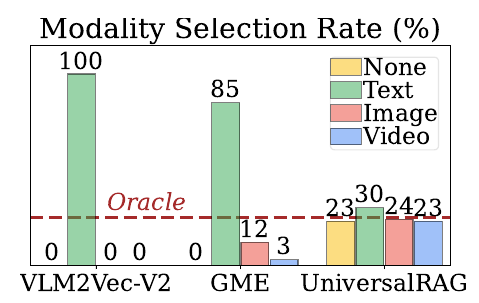
\includegraphics[width=\linewidth]{figures/tv1/universalrag-modality-dist.png}
    \caption{Tỷ lệ phương thức truy xuất (Hình~4 gốc).}
    \label{fig:tv1_modality_dist}
\end{subfigure}
\hfill
\begin{subfigure}[t]{0.32\textwidth}
    \centering
    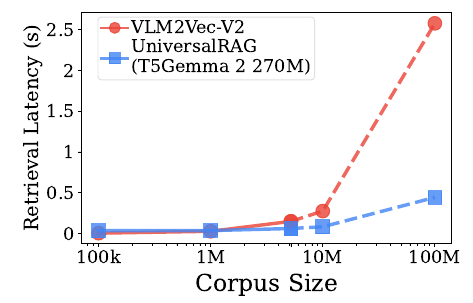
\includegraphics[width=\linewidth]{figures/tv1/universalrag-latency.png}
    \caption{Độ trễ theo quy mô kho (Hình~5 gốc).}
    \label{fig:tv1_latency}
\end{subfigure}
\hfill
\begin{subfigure}[t]{0.32\textwidth}
    \centering
    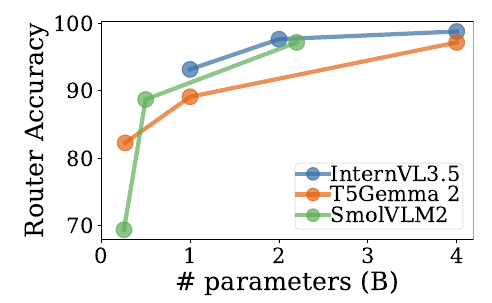
\includegraphics[width=\linewidth]{figures/tv1/universalrag-router-size.png}
    \caption{Độ chính xác theo cỡ router (Hình~6 gốc).}
    \label{fig:tv1_router_size}
\end{subfigure}
\caption[Phân tích tỷ lệ chọn phương thức, độ trễ truy vấn và kích thước bộ định tuyến của UniversalRAG]{Ba kết quả phân tích bổ sung của UniversalRAG \cite{yeo2026universalrag}: (a) tỷ lệ các phương thức được lấy ra trên 200 truy vấn mẫu mỗi tập; (b) thời gian truy xuất trung bình mỗi câu hỏi khi tăng quy mô kho từ 100k lên 100M mục (dùng router T5Gemma~2 270M); và (c) độ chính xác phân loại khi thay đổi kích thước router từ 256M đến 4B tham số.}
\label{fig:tv1_universalrag_analysis}
\end{figure}

Về tốc độ truy vấn, Hình~\ref{fig:tv1_universalrag_analysis}b kiểm chứng trực tiếp Mệnh đề~C.4: ở quy mô nhỏ (100k--1M mục), thời gian chạy bộ định tuyến $C$ làm cho UniversalRAG chậm tương đương hoặc nhỉnh hơn chút ít so với tìm trực tiếp. Tuy nhiên, khi tổng số mục tăng qua ngưỡng 10M lên tới 100M, độ trễ tìm kiếm trên kho gộp chung của VLM2Vec-V2 vọt lên gần 2,5 giây mỗi câu hỏi, trong khi UniversalRAG (dùng T5Gemma~2 270M) tăng chậm hơn nhiều nhờ chỉ phải tìm trên kho con đã chọn. Bên cạnh đó, Hình~\ref{fig:tv1_universalrag_analysis}c cho thấy độ chính xác định tuyến tăng theo số lượng tham số trên cả ba dòng mô hình (InternVL3.5, T5Gemma~2, SmolVLM2), nhưng ngay ở mốc 1B tham số đã đạt khoảng 90\%, đủ nhẹ để dùng làm bước tiền xử lý.

\paragraph{Khả năng tổng quát hóa trên dữ liệu ngoài phân phối (OOD) và kết hợp bộ định tuyến.}
Bảng~\ref{tab:universalrag_ood_ensemble} so sánh độ chính xác định tuyến trên cả 7 nhánh (\textit{Router Acc}, phân biệt với \textit{Modality Acc} 4 nhóm ở Bảng~\ref{tab:universalrag_routing_recall}) cùng điểm tạo sinh trung bình giữa 10 tập ID và 6 tập OOD.

\begin{table}[H]
\centering
\small
\caption[So sánh kết quả In-Domain và Out-of-Domain của UniversalRAG và các phương án kết hợp]{Độ chính xác định tuyến 7 nhánh (\textit{Router Acc}, \%) và điểm tạo sinh trung bình (Avg) trên 10 tập In-Domain và 6 tập Out-of-Domain với Qwen3-VL-8B-Instruct (Nguồn: Bảng~5 và Bảng~10 của \cite{yeo2026universalrag}).}
\label{tab:universalrag_ood_ensemble}
\renewcommand{\arraystretch}{1.20}
\begin{tabularx}{\textwidth}{@{}L *{4}{M{1.95cm}}@{}}
\toprule
\rowcolor{tblhead}
\thead{Phương pháp} & \thead{ID Router Acc} & \thead{ID Avg} & \thead{OOD Router Acc} & \thead{OOD Avg} \\
\midrule
Random (Chọn ngẫu nhiên 7 nhánh) & 14,29 & 31,75 & 14,29 & 37,85 \\
\rowcolor{zebrabg}
ParagraphRAG (Tốt nhất đơn kho, Bảng~10) & -- & 37,26 & -- & 42,62 \\
GME (Unified, Bảng~10) & -- & 33,88 & -- & 39,22 \\
\rowcolor{zebrabg}
$\mathrm{PE}_{\mathrm{core}}$ (Unified) & -- & 33,86 & -- & 39,08 \\
VLM2Vec-V2 (Unified) & -- & 33,31 & -- & 38,99 \\
\rowcolor{zebrabg}
MultiRAG (All corpora, Bảng~10) & -- & 34,07 & -- & 39,15 \\
\midrule
URAG (Qwen3-VL-2B, \textit{trained}) & 95,81 & 42,40 & 71,29 & 44,07 \\
\rowcolor{zebrabg}
URAG (InternVL3.5-1B, \textit{trained}) & 93,16 & 42,12 & 67,85 & 43,80 \\
URAG (T5Gemma 2 270M, \textit{trained}, Bảng~10) & -- & 41,68 & -- & 43,61 \\
\rowcolor{zebrabg}
URAG (GPT-5, \textit{training-free})$^{(*)}$ & 72,33 & 39,26 & 77,38 & 44,39 \\
URAG (Qwen3-VL-8B, \textit{training-free}, Bảng~10) & -- & 39,46 & -- & 44,35 \\
\midrule
\rowcolor{zebrabg}
Ensemble (Confidence-based) & 96,02 & 42,53 & \textbf{80,71} & \textbf{44,71} \\
Ensemble (Majority Voting) & \textbf{98,33} & \textbf{42,83} & 78,56 & 44,54 \\
\midrule
\rowcolor{zebrabg}
Oracle (Cận trên, Bảng~10) & -- & 42,45 & -- & 46,24 \\
\bottomrule
\end{tabularx}
\par\vspace{4pt}
{\footnotesize\raggedright\textit{Ghi chú:} $^{(*)}$ Trong bài báo gốc \cite{yeo2026universalrag}, điểm ID Avg của UniversalRAG (GPT-5) ghi là 39,26 ở Bảng~1 nhưng lại in là 41,68 ở Bảng~5; bảng trên giữ con số 39,26 khớp với các cột thành phần của Bảng~1 và nêu rõ điểm lệch này tại Mục~\ref{sec:exp_critique}.\par}
\end{table}

Số liệu ở Bảng~\ref{tab:universalrag_ood_ensemble} cho thấy sự khác biệt rõ giữa hai hướng thiết kế bộ định tuyến khi đổi miền dữ liệu. Trên 6 tập OOD chưa từng gặp lúc huấn luyện, độ chính xác định tuyến của Qwen3-VL-2B giảm 24,52 điểm phần trăm (từ 95,81\% xuống 71,29%), còn InternVL3.5-1B giảm 25,31 điểm (từ 93,16\% xuống 67,85%). Trái lại, bộ định tuyến dùng prompt GPT-5 không bị phụ thuộc vào phân phối huấn luyện nên đạt 77,38\% \textit{Router Acc} và 44,39 Avg trên OOD, vượt qua tất cả các bộ định tuyến đơn lẻ có huấn luyện (biến thể dùng prompt Qwen3-VL-8B cũng đạt tới 44,35 Avg ở Bảng~10). Khi ghép hai loại lại, phương án \textit{Confidence-based Ensemble} đạt kết quả OOD cao nhất với 80,71\% \textit{Router Acc} và 44,71 Avg (vượt mức tốt nhất của các baseline là ParagraphRAG 42,62 hay GME 39,22, tiến gần hơn tới Oracle 46,24), còn \textit{Majority Voting} đạt mức cao nhất trên ID với 98,33\% \textit{Router Acc} và 42,83 Avg.

\draftnote[TV3]{Tra cứu trực tiếp bản PDF gốc \textit{CoRe-MMRAG} (\texttt{2025.acl-long.1583}) để điền đầy đủ số liệu chính xác vào Bảng~\ref{tab:core_results}, ghi rõ tên MLLM nền và các baseline giải xung đột liên quan.}

\begin{table}[H]
\centering
\small
\caption[Kết quả thực nghiệm của CoRe-MMRAG trên các benchmark KB-VQA]{Kết quả thực nghiệm của CoRe-MMRAG trên các benchmark KB-VQA.}
\label{tab:core_results}
\renewcommand{\arraystretch}{1.24}
\begin{tabularx}{\textwidth}{@{}P{4.2cm}M{2.2cm}M{2.6cm}L@{}}
\toprule
\rowcolor{tblhead}
\thead{Phương pháp đối chứng} & \thead{InfoSeek} & \thead{Enc-VQA} & \thead{Ghi chú thiết lập} \\
\midrule
MLLM nền (No-RAG) & \dots & \dots & \dots \\
\rowcolor{zebrabg}
Standard Multimodal RAG & \dots & \dots & \dots \\
CoRe-MMRAG & \dots & \dots & \dots \\
\bottomrule
\end{tabularx}
\end{table}

% ------------------------------------------------------------------------------
\section{Kiểm chứng lập luận tác giả và đánh giá phản biện của nhóm}
\label{sec:exp_critique}

\draftnote[TV1 + TV2 + TV3]{Trả lời trực tiếp câu hỏi: ``Kết quả thực nghiệm có hỗ trợ những ưu điểm mà tác giả đưa ra không?'' và chỉ ra điểm yếu/đánh đổi ẩn ở từng bài:
(1) \textbf{ColPali}: Sụt mạnh ở 224$\times$224 (-24.8 điểm); Token Pooling giảm chất lượng trên trang chữ dày (\textit{Shift}); chưa đánh giá tạo sinh đầu--cuối; kiểm tra lại PDF gốc hai điểm lệch giữa văn bản Mục 6 và Bảng 7 (số patch ở 224$\times$224 và chiều biến thiên của \textit{No Q.A. Tokens} trên tiếng Pháp).
(2) \textbf{VisRAG}: Hiệu năng tạo sinh giảm khi tăng từ top-3 xuống top-10 do nhiễu đa trang; thiếu chứng minh lý thuyết về giới hạn 1 vector đơn.
(3) \textbf{UniversalRAG}: Giả định toán học còn lý tưởng; độ chính xác định tuyến OOD giảm so với ID.
(4) \textbf{CoRe-MMRAG}: Đánh đổi độ trễ suy luận 4 bước và bị giới hạn bởi năng lực đọc ảnh của MLLM nền.}

% TV1: Critical verification of UniversalRAG's claims and limitations
\paragraph{Kiểm chứng lập luận và đánh giá phản biện đối với UniversalRAG.}
Khi đối chiếu các tuyên bố của tác giả trong \cite{yeo2026universalrag} với số liệu ở Mục~\ref{subsec:quantitative_tables}, có thể thấy thực nghiệm đã chứng minh được ba kết luận chính: (i) tách riêng kho theo từng phương thức giúp tránh được hiện tượng thiên lệch về văn bản của không gian biểu diễn chung (\textit{Modality Acc} tăng từ 25,00\%--36,27\% lên 95,28\%, \textit{Recall}@5 tăng gấp đôi lên 44,82\% ở Bảng~3 và tỷ lệ chọn phương thức cân bằng trên Hình~4); (ii) cả hai cơ chế truy xuất liên phương thức và phân tách mức độ chi tiết đều mang lại cải thiện trên nhiều bộ dữ liệu và cả ba mô hình sinh LVLM (Bảng~2, 4, 8 và 9); và (iii) lợi thế về tốc độ tìm kiếm thể hiện rõ khi tổng quy mô kho vượt qua mốc 10M mục (Hình~5). Dù vậy, khi xét kỹ điều kiện thí nghiệm, phương pháp này vẫn còn bốn hạn chế và đánh đổi cần lưu ý:

\begin{enumerate}
    \item \textit{Giả định toán học đơn giản hóa nhiều so với dữ liệu thực}: Chứng minh Mệnh đề~2.1 và Mệnh đề~C.1 (Phụ lục~C.1) giả thiết các biến điểm số $X_c$ độc lập nhau, có kỳ vọng bằng 0, cùng tuân theo phân phối \textit{sub-Gaussian} với phương sai $\sigma^2$ như nhau trên mọi kho, rồi chặn trên bằng bất đẳng thức hợp (\textit{union bound}). Trong dữ liệu thực, các tài liệu cùng chủ đề có điểm tương đồng tương quan chặt với nhau và phân bố mật độ giữa kho ảnh, bảng và văn bản rất khác nhau. Tương tự, Mệnh đề~C.4 giả sử các kho con có cùng kích thước $N$ và việc truy vấn song song nhiều kho không gây tranh chấp tài nguyên phần cứng.
    \item \textit{Độ chính xác định tuyến giảm mạnh trên tập OOD và phụ thuộc nhiều vào GPT-4o}: Khi sang 6 tập OOD, độ chính xác của các bộ định tuyến có huấn luyện giảm khoảng 25 điểm phần trăm (Bảng~5: Qwen3-VL-2B giảm từ 95,81\% xuống 71,29\%; InternVL3.5-1B giảm từ 93,16\% xuống 67,85\%). Nguyên nhân chính đã được nhóm tác giả nêu trong mục \textit{Limitations}: hiện chưa có tập dữ liệu nào do con người gán nhãn phương thức và mức độ chi tiết cho từng câu hỏi. Nhãn huấn luyện được lấy tự động theo nguồn dữ liệu đích của từng tập, còn ở nhiều tập kiểm thử (LVBench, CinePile, WebQA, TriviaQA, VideoRAG), câu hỏi hoặc nhãn mức độ chi tiết đều do GPT-4o viết lại, lọc bớt hoặc phân loại tự động (Phụ lục~A.1--A.2, Hình~10--11). Cách chuẩn bị dữ liệu như vậy có thể làm câu hỏi mang văn phong gần với mô hình ngôn ngữ lớn, gián tiếp có lợi cho bộ định tuyến dùng prompt.
    \item \textit{Chia quá nhiều mức chi tiết không phải lúc nào cũng tăng điểm và dễ nhầm ở vùng giáp ranh}: Trên HotpotQA với GPT-5 (Bảng~4), khi tăng số mức chi tiết $\#\mathrm{Gn}$ từ 2 lên 3 thì điểm EM giảm nhẹ từ 24,35 xuống 24,20 rồi mới tăng lại ở $\#\mathrm{Gn}=4$. Nguyên nhân là khi chia nhỏ thêm các mức \textit{Passage} và \textit{Section}, ranh giới định nghĩa giữa các mức gần nhau trở nên khó phân biệt hơn. Năm ví dụ lỗi tại Bảng~15 của bài gốc cũng cho thấy bộ định tuyến dễ nhầm ở các câu hỏi giáp ranh (chọn \textit{No} thay vì \textit{Paragraph} cho câu hỏi về nguồn gốc từ vựng, nhầm \textit{Clip} sang \textit{Image} hoặc \textit{Video}, và thiếu nhánh \textit{Image} khi câu hỏi cần \textit{Paragraph+Image}), bên cạnh việc phụ thuộc vào ngưỡng xác suất cố định 0,8 ở bước suy luận đa nhãn (Phụ lục~B).
    \item \textit{Chi phí xây dựng hệ thống đa chỉ mục và giới hạn của thiết kế thí nghiệm}: Để vận hành UniversalRAG, hệ thống phải lập và bảo trì đồng thời 6 chỉ mục riêng, nạp 3 bộ mã hóa khác nhau (Qwen3-Embedding-4B, VLM2Vec-V2 và biểu diễn vector đặc theo từng hàng của bảng), đồng thời chạy nhiều bước tiền xử lý ngoại tuyến như cắt cảnh video bằng PySceneDetect, lấy mẫu 32 khung hình và sinh mô tả ảnh, lời thoại video để tính điểm kết hợp theo tỷ lệ 0,8/0,2 (Phụ lục~B). Phần chi phí lưu trữ và tiền xử lý này không nằm trong phép đo thời gian truy vấn ở Hình~5. Ngoài ra, mọi con số thực nghiệm chỉ chạy một lần duy nhất (Phụ lục~A.3) nên không có độ lệch chuẩn để đánh giá mức dao động, và có một điểm không khớp nhỏ giữa Bảng~1 với Bảng~5 của bài gốc ở điểm trung bình ID của UniversalRAG (GPT-5) (Bảng~1 ghi 39,26 nhưng Bảng~5 ghi 41,68, trùng với điểm của T5Gemma~2 270M ở Bảng~1). Từ đó có thể thấy UniversalRAG phù hợp nhất khi kho dữ liệu thực sự lớn, trải trên nhiều phương thức và có dùng kết hợp bộ định tuyến (\textit{Ensemble}) để tránh sụt giảm khi gặp câu hỏi mới.
\end{enumerate}


% Optional bonus chapter for code reproduction and error analysis (comment out if omitted)
% ==============================================================================
% Chapter 5: Optional Mini-Reproduction & Error Analysis (Clean Skeleton)
% Note: Comment out % ==============================================================================
% Chapter 5: Optional Mini-Reproduction & Error Analysis (Clean Skeleton)
% Note: Comment out % ==============================================================================
% Chapter 5: Optional Mini-Reproduction & Error Analysis (Clean Skeleton)
% Note: Comment out \input{chapters/05_reproduction} in main.tex if omitted
% ==============================================================================

\chapter{Thực nghiệm kiểm chứng và phân tích lỗi}
\label{chap:reproduction}

\draftnote[Chung]{Chương 5 là phần TÙY CHỌN để lấy điểm cộng (``không bắt buộc, nhưng chạy lại được và có đánh giá về tốc độ, kết quả, phân tích lỗi là điểm cộng''). Nếu nhóm không chạy code thực tế, hãy comment dòng nạp tệp \texttt{chapters/05\_reproduction} trong \texttt{main.tex} và tăng chiều sâu phân tích ví dụ định tính từ phụ lục bài báo ở Chương 3--4.}

% ------------------------------------------------------------------------------
\section{Thiết lập môi trường và tập dữ liệu kiểm thử}
\label{sec:repro_setup}

\draftnote[TV2 + TV1]{Mô tả phần cứng (ví dụ GPU Google Colab T4/L4), phiên bản mã nguồn mở (ví dụ \texttt{colpali-engine}, \texttt{OpenBMB/visrag}), và tập mẫu 20--50 trang PDF đa phương thức dùng để đối chứng TextRAG (OCR + BGE-M3/BM25) với Vision-space RAG.}

% ------------------------------------------------------------------------------
\section{Đánh giá thực tế về tốc độ, bộ nhớ và độ chính xác}
\label{sec:repro_metrics}

\draftnote[TV2]{Ghi lại kết quả đo thực tế vào Bảng~\ref{tab:repro_benchmark} và nhận xét mức độ nhất quán với kết quả công bố trong bài báo gốc.}

\begin{table}[H]
\centering
\small
\caption[Kết quả đo thực nghiệm đối chứng trên tập kiểm thử nội bộ]{Kết quả đo thực nghiệm đối chứng trên tập kiểm thử nội bộ của nhóm.}
\label{tab:repro_benchmark}
\renewcommand{\arraystretch}{1.24}
\begin{tabularx}{\textwidth}{@{}L M{1.95cm} M{1.7cm} M{2.05cm} M{2.0cm}@{}}
\toprule
\rowcolor{tblhead}
\thead{Pipeline thử nghiệm} & \thead{Indexing\newline (s/trang)} & \thead{Query\newline (ms)} & \thead{Dung lượng\newline chỉ mục} & \thead{Recall\newline @1 / @5} \\
\midrule
TextRAG (OCR + \dots) & \dots & \dots & \dots & \dots \\
\rowcolor{zebrabg}
ColPali / ColQwen2 & \dots & \dots & \dots & \dots \\
VisRAG-Ret & \dots & \dots & \dots & \dots \\
\bottomrule
\end{tabularx}
\end{table}

% ------------------------------------------------------------------------------
\section{Phân tích lỗi định tính (Error Analysis)}
\label{sec:repro_error_analysis}

\draftnote[TV3]{Trình bày 2--3 tình huống cụ thể kèm ảnh chụp minh họa: (1) Ca TextRAG lỗi do OCR/bố cục nhưng Vision-space RAG đúng; (2) Bản đồ nhiệt MaxSim của ColPali định vị vùng đồ thị/bảng biểu; (3) Ca thất bại thực tế của Vision-space RAG (chữ quá nhỏ hoặc nhiễu khi nhiều trang).}
 in main.tex if omitted
% ==============================================================================

\chapter{Thực nghiệm kiểm chứng và phân tích lỗi}
\label{chap:reproduction}

\draftnote[Chung]{Chương 5 là phần TÙY CHỌN để lấy điểm cộng (``không bắt buộc, nhưng chạy lại được và có đánh giá về tốc độ, kết quả, phân tích lỗi là điểm cộng''). Nếu nhóm không chạy code thực tế, hãy comment dòng nạp tệp \texttt{chapters/05\_reproduction} trong \texttt{main.tex} và tăng chiều sâu phân tích ví dụ định tính từ phụ lục bài báo ở Chương 3--4.}

% ------------------------------------------------------------------------------
\section{Thiết lập môi trường và tập dữ liệu kiểm thử}
\label{sec:repro_setup}

\draftnote[TV2 + TV1]{Mô tả phần cứng (ví dụ GPU Google Colab T4/L4), phiên bản mã nguồn mở (ví dụ \texttt{colpali-engine}, \texttt{OpenBMB/visrag}), và tập mẫu 20--50 trang PDF đa phương thức dùng để đối chứng TextRAG (OCR + BGE-M3/BM25) với Vision-space RAG.}

% ------------------------------------------------------------------------------
\section{Đánh giá thực tế về tốc độ, bộ nhớ và độ chính xác}
\label{sec:repro_metrics}

\draftnote[TV2]{Ghi lại kết quả đo thực tế vào Bảng~\ref{tab:repro_benchmark} và nhận xét mức độ nhất quán với kết quả công bố trong bài báo gốc.}

\begin{table}[H]
\centering
\small
\caption[Kết quả đo thực nghiệm đối chứng trên tập kiểm thử nội bộ]{Kết quả đo thực nghiệm đối chứng trên tập kiểm thử nội bộ của nhóm.}
\label{tab:repro_benchmark}
\renewcommand{\arraystretch}{1.24}
\begin{tabularx}{\textwidth}{@{}L M{1.95cm} M{1.7cm} M{2.05cm} M{2.0cm}@{}}
\toprule
\rowcolor{tblhead}
\thead{Pipeline thử nghiệm} & \thead{Indexing\newline (s/trang)} & \thead{Query\newline (ms)} & \thead{Dung lượng\newline chỉ mục} & \thead{Recall\newline @1 / @5} \\
\midrule
TextRAG (OCR + \dots) & \dots & \dots & \dots & \dots \\
\rowcolor{zebrabg}
ColPali / ColQwen2 & \dots & \dots & \dots & \dots \\
VisRAG-Ret & \dots & \dots & \dots & \dots \\
\bottomrule
\end{tabularx}
\end{table}

% ------------------------------------------------------------------------------
\section{Phân tích lỗi định tính (Error Analysis)}
\label{sec:repro_error_analysis}

\draftnote[TV3]{Trình bày 2--3 tình huống cụ thể kèm ảnh chụp minh họa: (1) Ca TextRAG lỗi do OCR/bố cục nhưng Vision-space RAG đúng; (2) Bản đồ nhiệt MaxSim của ColPali định vị vùng đồ thị/bảng biểu; (3) Ca thất bại thực tế của Vision-space RAG (chữ quá nhỏ hoặc nhiễu khi nhiều trang).}
 in main.tex if omitted
% ==============================================================================

\chapter{Thực nghiệm kiểm chứng và phân tích lỗi}
\label{chap:reproduction}

\draftnote[Chung]{Chương 5 là phần TÙY CHỌN để lấy điểm cộng (``không bắt buộc, nhưng chạy lại được và có đánh giá về tốc độ, kết quả, phân tích lỗi là điểm cộng''). Nếu nhóm không chạy code thực tế, hãy comment dòng nạp tệp \texttt{chapters/05\_reproduction} trong \texttt{main.tex} và tăng chiều sâu phân tích ví dụ định tính từ phụ lục bài báo ở Chương 3--4.}

% ------------------------------------------------------------------------------
\section{Thiết lập môi trường và tập dữ liệu kiểm thử}
\label{sec:repro_setup}

\draftnote[TV2 + TV1]{Mô tả phần cứng (ví dụ GPU Google Colab T4/L4), phiên bản mã nguồn mở (ví dụ \texttt{colpali-engine}, \texttt{OpenBMB/visrag}), và tập mẫu 20--50 trang PDF đa phương thức dùng để đối chứng TextRAG (OCR + BGE-M3/BM25) với Vision-space RAG.}

% ------------------------------------------------------------------------------
\section{Đánh giá thực tế về tốc độ, bộ nhớ và độ chính xác}
\label{sec:repro_metrics}

\draftnote[TV2]{Ghi lại kết quả đo thực tế vào Bảng~\ref{tab:repro_benchmark} và nhận xét mức độ nhất quán với kết quả công bố trong bài báo gốc.}

\begin{table}[H]
\centering
\small
\caption[Kết quả đo thực nghiệm đối chứng trên tập kiểm thử nội bộ]{Kết quả đo thực nghiệm đối chứng trên tập kiểm thử nội bộ của nhóm.}
\label{tab:repro_benchmark}
\renewcommand{\arraystretch}{1.24}
\begin{tabularx}{\textwidth}{@{}L M{1.95cm} M{1.7cm} M{2.05cm} M{2.0cm}@{}}
\toprule
\rowcolor{tblhead}
\thead{Pipeline thử nghiệm} & \thead{Indexing\newline (s/trang)} & \thead{Query\newline (ms)} & \thead{Dung lượng\newline chỉ mục} & \thead{Recall\newline @1 / @5} \\
\midrule
TextRAG (OCR + \dots) & \dots & \dots & \dots & \dots \\
\rowcolor{zebrabg}
ColPali / ColQwen2 & \dots & \dots & \dots & \dots \\
VisRAG-Ret & \dots & \dots & \dots & \dots \\
\bottomrule
\end{tabularx}
\end{table}

% ------------------------------------------------------------------------------
\section{Phân tích lỗi định tính (Error Analysis)}
\label{sec:repro_error_analysis}

\draftnote[TV3]{Trình bày 2--3 tình huống cụ thể kèm ảnh chụp minh họa: (1) Ca TextRAG lỗi do OCR/bố cục nhưng Vision-space RAG đúng; (2) Bản đồ nhiệt MaxSim của ColPali định vị vùng đồ thị/bảng biểu; (3) Ca thất bại thực tế của Vision-space RAG (chữ quá nhỏ hoặc nhiễu khi nhiều trang).}


% ==============================================================================
% Chapter 6: Conclusion, Research Trends, and Open Gaps
% Owner: Member 2 (TV2)
% ==============================================================================

\chapter{Kết luận, xu hướng và khoảng trống nghiên cứu}
\label{chap:conclusion}

\section{Tổng kết các phát hiện chính của báo cáo}
\label{sec:conc_summary}

Bài khảo sát \textit{Ask in Any Modality} đặt Multimodal RAG trong
một khung gồm các lựa chọn về truy xuất, kết hợp thông tin, tăng cường
ngữ cảnh, tạo sinh và huấn luyện. Khung này giúp xác định công đoạn mà
mỗi nghiên cứu cải thiện và điều kiện để chuyển kết quả của nghiên
cứu vào một hệ thống khác \cite{abootorabi2025ask}. Ba thông điệp ở
slide kết luận của nhóm tập trung vào đường đi của chứng cứ từ kho
dữ liệu đến câu trả lời.

\paragraph{Ảnh trang giữ chứng cứ về bố cục.}
ColPali và VisRAG cho thấy trang PDF có thể được lập chỉ mục trực
tiếp dưới dạng ảnh. Trên ViDoRe, ColPali cải thiện nDCG@5 trung bình
từ 66,1 của BGE-M3 + OCR lên 81,3. Các mức tăng lớn ở hình khoa học
và infographic cho thấy có những trường hợp việc giữ bố cục ảnh
làm thay đổi đáng kể kết quả tìm trang. Ở tầng sinh, ví dụ LinkedIn
trong bài VisRAG cho thấy cả hai pipeline có thể chọn đúng cùng
một trang nhưng chỉ cấu hình đọc ảnh gắn đúng tỷ lệ với vùng địa
lý. Cần đánh giá tìm trang và đọc chứng cứ bằng các phép đo riêng
\cite{faysse2025colpali,yu2025visrag}.

Khả năng đọc bố cục có chi phí. ColPali lưu khoảng 1030 vector
128 chiều cho một trang và so khớp từng token truy vấn. VisRAG-Ret
lưu một vector 2304 chiều, thuận tiện cho chỉ mục vector. Điểm
MRR@10 của VisRAG-Ret nhỉnh hơn trung bình trong phép đối chiếu
sáu tập, còn ColPali có lợi thế trên DocVQA và SlideVQA trong
cùng thiết lập. Một hệ thống dùng nhiều vector có thể đầu tư vào
độ phân giải và khả năng kiểm tra vùng khớp. Một hệ thống dùng
vector đơn có thể dùng phần tài nguyên tiết kiệm để duy trì kho
lớn hơn hoặc cấp thêm ứng viên cho bộ đọc. Việc chọn cấu hình cần
gắn với truy vấn thực tế, ngân sách bộ nhớ và yêu cầu độ trễ
\cite{faysse2025colpali,yu2025visrag}.

\paragraph{Định tuyến theo phương thức và độ chi tiết.}
Một kho có văn bản, bảng, ảnh và video đặt ra câu hỏi trước khi
xếp hạng. Hệ thống phải xác định loại dữ liệu có thể trả lời
và mức chi tiết thích hợp. Ví dụ, câu hỏi về một sự kiện ngắn cần
ứng viên ở cấp clip, còn câu hỏi về bố cục của cả một báo cáo có
thể cần tài liệu đầy đủ. UniversalRAG dùng bộ định tuyến chọn kho
theo phương thức và độ chi tiết. Kết quả gần Oracle trong thiết
lập được trình bày ở slide 15 cho thấy tiềm năng của việc chọn
kho trước khi so khớp. Điểm Oracle chỉ là mốc tham chiếu trong
thiết lập đó. Ở miền mới, sai số định tuyến có thể loại chứng cứ
trước khi bộ truy xuất có cơ hội xếp hạng \cite{yeo2026universalrag}.

\paragraph{Đối soát khi chứng cứ không nhất quán.}
Khi bộ sinh có câu trả lời từ tri thức tham số và đồng thời đọc
chứng cứ bên ngoài, hai nguồn có thể dẫn đến các đáp án khác nhau.
Ảnh và văn bản trong tập truy xuất cũng có thể chỉ đến các thực
thể khác nhau. CoRe-MMRAG coi những trường hợp này là hai dạng
xung đột PRKI và VTKI, rồi đối soát qua nhiều bước. Ví dụ máy bay
trong slide đặt ra cả việc nhận đúng thực thể từ ảnh lẫn việc
xác nhận mốc thời gian từ nguồn ngoài. Giá trị của cơ chế đối
soát phụ thuộc vào độ bao phủ và chất lượng của chứng cứ được
truy xuất. Nếu cả tập trang đều bỏ sót chứng cứ cần thiết, nên
ghi nhận thiếu căn cứ để trả lời \cite{tian2025coremmrag}.

Khi ghép các ý trên thành một pipeline, có thể theo dõi lỗi theo
thứ tự. Tầng định tuyến chọn kho, tầng truy xuất chọn chứng cứ
trong kho, tầng đọc và đối soát dùng chứng cứ để tạo đáp án.
Một câu trả lời có thể sai do bất kỳ bước nào, và lỗi ở bước
trước làm giảm khả năng sửa lỗi ở bước sau. Vì vậy, báo cáo độ
chính xác đầu cuối cần đi cùng dấu vết của kho đã chọn, mã trang
đã truy xuất và nguồn dùng để suy luận. Các kết quả nghiên cứu
hiện tại minh họa từng tầng dưới những bộ dữ liệu và chỉ số cụ
thể.

\section{Các xu hướng nghiên cứu chủ đạo}
\label{sec:conc_trends}

\paragraph{Cải thiện VLM làm nền cho truy xuất.}
Slide 17 nêu bước chuyển từ PaliGemma sang Qwen2-VL. Biến thể
ColQwen2 đạt 86,6 nDCG@5 so với 81,3 của ColPali tham chiếu,
tăng 5,3 điểm trong Bảng 7 của nghiên cứu. ColQwen2 dùng chiến
lược huấn luyện tương tự và giới hạn số mảnh ảnh ở 768 để gần
mức bộ nhớ của cấu hình tham chiếu. Đây là bằng chứng về khả
năng thích ứng của cơ chế late interaction khi bộ mã hóa thị
giác--ngôn ngữ mạnh hơn. Số mảnh ảnh và backbone thay đổi cùng
lúc, nên muốn giải thích riêng phần cải thiện do backbone cần
thêm đối chứng \cite{faysse2025colpali}.

Một hệ quả của xu hướng này là nên đánh giá backbone qua kiểu
chứng cứ và điều kiện sử dụng. OCR nội tại của VLM có thể giúp
khớp chữ từ ảnh, nhưng năng lực đó cần đo riêng trên bản quét,
chữ nhỏ và ngôn ngữ ngoài tập huấn luyện. Với biểu đồ, hiểu vị
trí của trục, chú giải và các điểm còn quan trọng hơn tìm được
từ khóa. Hệ thống có thể đạt chất lượng truy xuất tốt mà vẫn
phải thêm bước đọc vùng có độ phân giải cao để trả lời các câu
hỏi về giá trị chính xác.

\paragraph{Duy trì ảnh qua cả truy xuất lẫn tạo sinh.}
VisRAG minh họa xu hướng giữ ảnh làm biểu diễn trung gian từ lập
chỉ mục đến khi chuyển ngữ cảnh cho bộ sinh. Ở đây ảnh là đầu
vào chứng cứ còn câu trả lời có thể ở dạng văn bản. Khái niệm
pipeline thị giác trong slide đề cập đường đi của dữ liệu tài
liệu. Cách này giữ được quan hệ giữa nội dung và bố cục tới khi
bộ sinh đọc trang. Các cơ chế đọc nhiều ảnh mở rộng phép đối
chiếu từ một trang sang nhiều trang \cite{yu2025visrag}.

Một thiết kế ứng dụng có thể giữ mã tài liệu, số trang và ảnh
cùng với biểu diễn dùng để tìm kiếm. Khi phát hiện một kết quả
nhạy với chữ nhỏ, hệ thống có thể chuyển ảnh cắt vùng tương ứng
cho bộ sinh trong khi vẫn bảo toàn thông tin nguồn. Tầng truy
xuất có thể đi từ trang đến vùng, còn tầng sinh cần nối kết quả
với mã trang để người đọc kiểm tra. Những lựa chọn này cần được
đánh giá về độ bao phủ lẫn chi phí xử lý các ảnh bổ sung.

\section{Các khoảng trống nghiên cứu (Research Gaps) còn tồn tại}
\label{sec:conc_gaps}

\subsubsection{Nén chỉ mục đa vector ở quy mô lớn}

Khi một trang có hơn một nghìn vector, chênh lệch dung lượng
nhanh chóng tăng cùng số trang. Nén theo nhóm có thể giảm lặp ở
các vùng nền và giảm chi phí xếp hạng. Nút thắt nằm ở các vùng
nhỏ nhưng chứa đủ chứng cứ, chẳng hạn một ô ghi tỷ lệ trong bảng.
Kết quả token pooling của ColPali cho thấy điểm trung bình giữ
được 97,8\% ở hệ số 3, nhưng các trang dày chữ trong Shift nhạy
hơn với nén \cite{faysse2025colpali}.

Một thí nghiệm tiếp theo có thể chia tập truy vấn theo chứng cứ
cần đọc và thay đổi hệ số gộp theo từng mức. Với mỗi mức, ghi
nDCG, Recall, dung lượng đã lưu, độ trễ truy vấn ở phân vị 95
và tốc độ bổ sung trang mới. Cần ghi thêm trường hợp trang đúng
rơi khỏi danh sách ứng viên sau nén. Tập có nhiều biểu đồ và
tập có nhiều bảng chữ nhỏ nên được báo cáo riêng để xem cùng
một cấu hình phù hợp cho bao nhiêu loại tài liệu.

\subsubsection{Suy luận nhiều trang và nhiều bước}

Một câu hỏi nhiều bước có thể yêu cầu đọc một số liệu, tìm đơn
vị ở trang khác rồi thực hiện phép tính. Nếu chỉ chấm việc tìm
một trang đúng, phép đánh giá có thể bỏ qua việc hệ thống thiếu
phần chứng cứ còn lại. Nếu chỉ chấm kết quả, đáp án đúng do
suy đoán có thể được tính ngang với đáp án kiểm chứng được.
Có thể gán nhãn tập trang cần dùng và kiểm tra cả độ bao phủ
chứng cứ lẫn sự đúng đắn của phép nối thông tin.

Khi tăng số ảnh trong ngữ cảnh, mô hình có thể thấy nhiều chứng
cứ hơn nhưng cũng có thể chọn nhầm trang gần chủ đề. Bảng 3
của VisRAG cho thấy lợi ích trung bình của cấu hình đa ảnh từ
top-1 đến top-3, cùng sự khác biệt theo bộ dữ liệu. Một thí
nghiệm có thể cố định trang đúng và thay đổi số trang nhiễu,
thứ tự trang, độ phân giải và vị trí xuất hiện của chứng cứ.
Kết quả cần ghi cả thời gian sinh, độ chính xác câu trả lời
và tỷ lệ chỉ đúng các trang dùng để suy luận \cite{yu2025visrag}.

\subsubsection{Định vị chứng cứ theo thời gian trong video dài}

Slide 17 đặt temporal grounding như giới hạn của truy xuất thị
giác ở quy mô lớn. Một clip ngắn thuận tiện cho xác định khung
hình chứa sự kiện, nhưng có thể bỏ mất thông tin ngay trước hoặc
sau mốc đó. Cửa sổ dài giữ nhiều bối cảnh và cần nhiều tài nguyên
hơn khi chấm điểm hoặc đưa vào mô hình. UniversalRAG minh họa
việc chọn giữa clip và video ở tầng định tuyến
\cite{yeo2026universalrag}. Sau khi kho đã được chọn, vẫn cần
xác định mốc thời gian thực sự hỗ trợ câu trả lời.

Thử nghiệm trên video dài có thể đánh giá hai tầng. Tầng đầu
truy xuất video hoặc cụm clip. Tầng sau tinh chỉnh vị trí đoạn
liên quan. Cần ghi độ bao phủ video đúng, mức trùng khớp của
đoạn thời gian và chi phí tính toán trên mỗi giờ video.
Với một câu cần hai sự kiện cách xa nhau, điều kiện thành công
phải yêu cầu tìm được cả hai mốc. Cách đánh giá này song song với
bài toán tìm đủ trang trong tài liệu nhiều trang.

\subsubsection{Chuyển miền sang tài liệu tiếng Việt và bản quét}

Kết quả từ ViDoRe và sáu tập của VisRAG tạo cơ sở để chọn
cấu hình thử nghiệm. Khi áp dụng vào tài liệu tiếng Việt,
cần kiểm tra lại khả năng đọc dấu, nhận dạng chữ nhỏ và
liên kết ô bảng với tiêu đề. Chẳng hạn, hồ sơ hành chính
có thể chứa con dấu chồng lên tên đơn vị, còn báo cáo tài
chính có cột đơn vị ghi ở chú thích riêng. Cả hai đều
chứa chữ và bố cục, nhưng cách làm hỏng chứng cứ khác
nhau. Một phép đo theo nhóm bản quét, PDF sinh từ máy và
tài liệu nhiều bảng sẽ cho biết mức độ chuyển miền rõ
hơn so với một điểm trung bình duy nhất.

Tiếng Việt cũng đặt ra yêu cầu về cách viết câu hỏi.
Một mã biểu mẫu có thể xuất hiện cùng cách gọi tắt ở
phần đầu và tên đầy đủ ở phần phụ lục. Người dùng có
thể hỏi bằng tên tắt, cách gõ có dấu hoặc dạng thiếu dấu.
Có thể giữ nguyên trang chứng cứ rồi tạo các biến thể
câu hỏi phù hợp với thói quen tra cứu. Đo vị trí của cùng
một trang qua các biến thể giúp tách lỗi ở biểu diễn
truy vấn khỏi lỗi do độ phân giải và bố cục trang. Đối
với tìm mã, điểm thành công cần xét đúng từng ký tự.
Đối với tìm chủ đề, người đánh giá có thể chấp nhận các
trang khác nếu chúng chứa đủ chứng cứ cho câu trả lời.

Một thiết lập kiểm tra chất lượng ảnh có thể giữ cùng
PDF, trang và truy vấn, rồi so sánh ảnh gốc với phiên
bản giảm độ phân giải hoặc nghiêng nhẹ. Với ColPali, theo
dõi trang đúng và độ ổn định của các vùng đạt điểm
MaxSim cao. Với VisRAG, giữ nguyên danh sách trang
Oracle khi đo khả năng đọc của bộ sinh, sau đó đo lại
trong chế độ truy xuất thực tế. Nếu điểm Oracle giảm khi
thay chất lượng ảnh, lỗi đọc vẫn tồn tại dù đã tìm đúng
trang. Nếu Oracle ổn định nhưng Recall giảm, bước lập
chỉ mục hoặc khớp truy vấn cần được xem xét trước. Cách
bố trí này kiểm tra trực tiếp các giả thuyết về ảnh
trang và lỗi lan truyền ở slide 7, 8 và 16.

Trong một kho thật, lỗi điển hình có thể hiếm nhưng gây
hậu quả lớn, chẳng hạn đọc nhầm một chữ số hoặc đơn vị
trong bảng công nợ. Bộ thử nên ghi đồng thời tỷ lệ tìm
đúng trang, tỷ lệ đọc chính xác giá trị và tỷ lệ dẫn được
chứng cứ. Kết quả cần chỉ ra nhóm nào chịu ảnh hưởng khi
nén chỉ mục hoặc giới hạn số ảnh, rồi đối chiếu mức tiết
kiệm bộ nhớ và thời gian của cấu hình tương ứng. Đây là
một hướng kiểm chứng cho báo cáo, với thí nghiệm gốc của
ColPali và VisRAG làm mốc tham khảo
\cite{faysse2025colpali,yu2025visrag}.

Một câu hỏi chung của ba hướng là hệ thống có thể cung cấp đủ
chứng cứ trong giới hạn thời gian và bộ nhớ hay không. Phép đo
trên một tập truy vấn thống nhất cần ghi rõ kho đã chọn, tập
trang hoặc đoạn đã lấy, chất lượng câu trả lời và thời gian đầu
cuối. Những chỉ số đó cho phép gắn kết quả của từng tầng với
lợi ích quan sát được đối với người đọc.


% ------------------------------------------------------------------------------
% References (IEEEtran BibTeX, listed in Table of Contents)
% In draft mode, display the 5 core papers in References until inline \cite{} is added
% ------------------------------------------------------------------------------
\clearpage
\phantomsection
\addcontentsline{toc}{chapter}{\bibname}
\ifshowdraftnotes
    \nocite{abootorabi2025ask,yeo2026universalrag,faysse2025colpali,yu2025visrag,tian2025coremmrag}
\fi
\bibliographystyle{IEEEtran}
\bibliography{references}

\end{document}
